\documentclass[11pt]{article}
	\usepackage[T1]{fontenc}
    % Nicer default font (+ math font) than Computer Modern for most use cases
    % \usepackage{mathpazo}

    % Basic figure setup, for now with no caption control since it's done
    % automatically by Pandoc (which extracts ![](path) syntax from Markdown).
    \usepackage{graphics}
    % We will generate all images so they have a width \maxwidth. This means
    % that they will get their normal width if they fit onto the page, but
    % are scaled down if they would overflow the margins.
    \makeatletter
    \def\maxwidth{\ifdim\Gin@nat@width>\linewidth\linewidth
    \else\Gin@nat@width\fi}
    \makeatother
    \let\Oldincludegraphics\includegraphics
    % Set max figure width to be 80% of text width, for now hardcoded.
    \renewcommand{\includegraphics}[1]{\Oldincludegraphics[width=.8\maxwidth]{#1}}
    % Ensure that by default, figures have no caption (until we provide a
    % proper Figure object with a Caption API and a way to capture that
    % in the conversion process - todo).
    \usepackage[center,bf]{caption}
    % \DeclareCaptionLabelFormat{nolabel}{}
    % \captionsetup{labelformat=nolabel}

    \usepackage{adjustbox} % Used to constrain images to a maximum size 
    \usepackage{xcolor} % Allow colors to be defined
    \usepackage{enumerate} % Needed for markdown enumerations to work
    \usepackage{geometry} % Used to adjust the document margins
    \usepackage{amsmath} % Equations
    \usepackage{amssymb} % Equations
    \usepackage{textcomp} % defines textquotesingle
    % Hack from http://tex.stackexchange.com/a/47451/13684:
    \AtBeginDocument{%
        \def\PYZsq{\textquotesingle}% Upright quotes in Pygmentized code
    }
    \usepackage{upquote} % Upright quotes for verbatim code
    \usepackage{eurosym} % defines \euro
    \usepackage[mathletters]{ucs} % Extended unicode (utf-8) support
    \usepackage[utf8x]{inputenc} % Allow utf-8 characters in the tex document
    \usepackage{fancyvrb} % verbatim replacement that allows latex
    \usepackage{grffile} % extends the file name processing of package graphics 
                         % to support a larger range 
    % The hyperref package gives us a pdf with properly built
    % internal navigation ('pdf bookmarks' for the table of contents,
    % internal cross-reference links, web links for URLs, etc.)
    \usepackage{hyperref}
    \usepackage{longtable} % longtable support required by pandoc >1.10
    \usepackage{booktabs}  % table support for pandoc > 1.12.2
    \usepackage[inline]{enumitem} % IRkernel/repr support (it uses the enumerate* environment)
    \usepackage[normalem]{ulem} % ulem is needed to support strikethroughs (\sout)
                                % normalem makes italics be italics, not underlines
   	\usepackage[]{authblk}
   	\usepackage{cite}
    \usepackage{graphicx}
    \usepackage{hyperref}
    \usepackage{amsmath}
    \usepackage{amsthm}
    \usepackage{amssymb}
    \usepackage{bm}
    \usepackage{bbm}
    \usepackage{algorithmicx}
    \usepackage{algorithm}
    \usepackage{algpseudocode}
    \usepackage{array}
    \usepackage{booktabs}
    \usepackage{multirow}
    \usepackage{makecell}
    \usepackage{color}
    \usepackage{tabularx,ragged2e,booktabs,caption}

   	\makeatletter
    \def\@maketitle{%
    \newpage
      \null
      \vskip 2em%
      \begin{center}%
      \let \footnote \thanks
        {\Large\bfseries \@title \par}%
        \vskip 1.5em%
        {\normalsize
          \lineskip .5em%
          \begin{tabular}[t]{c}%
            \@author
          \end{tabular}\par}%
        \vskip 1em%
        {\normalsize \@date}%
      \end{center}%
      \par
      \vskip 1.5em}
    \makeatother


\newtheorem{theorem}{Theorem}






\title{EE 232E Project 2\\Social Network Mining}
\author{Hengjie~Yang, Sheng~Chang, Wendi~Cui, and Tianyi~Liu
}


\date{\today}


\begin{document}
\maketitle

\section{A brief tutorial on how to use this template}
\Large\textcolor{red}{\bf{Please remove the tutorial section in the final manuscript\\ by commenting, i.e. $\%(something)$}}


\subsection{Figures}
Figure insertion is shown in Fig \ref{example_fig}.
\begin{figure}[h]
\centering
\scalebox{0.7}{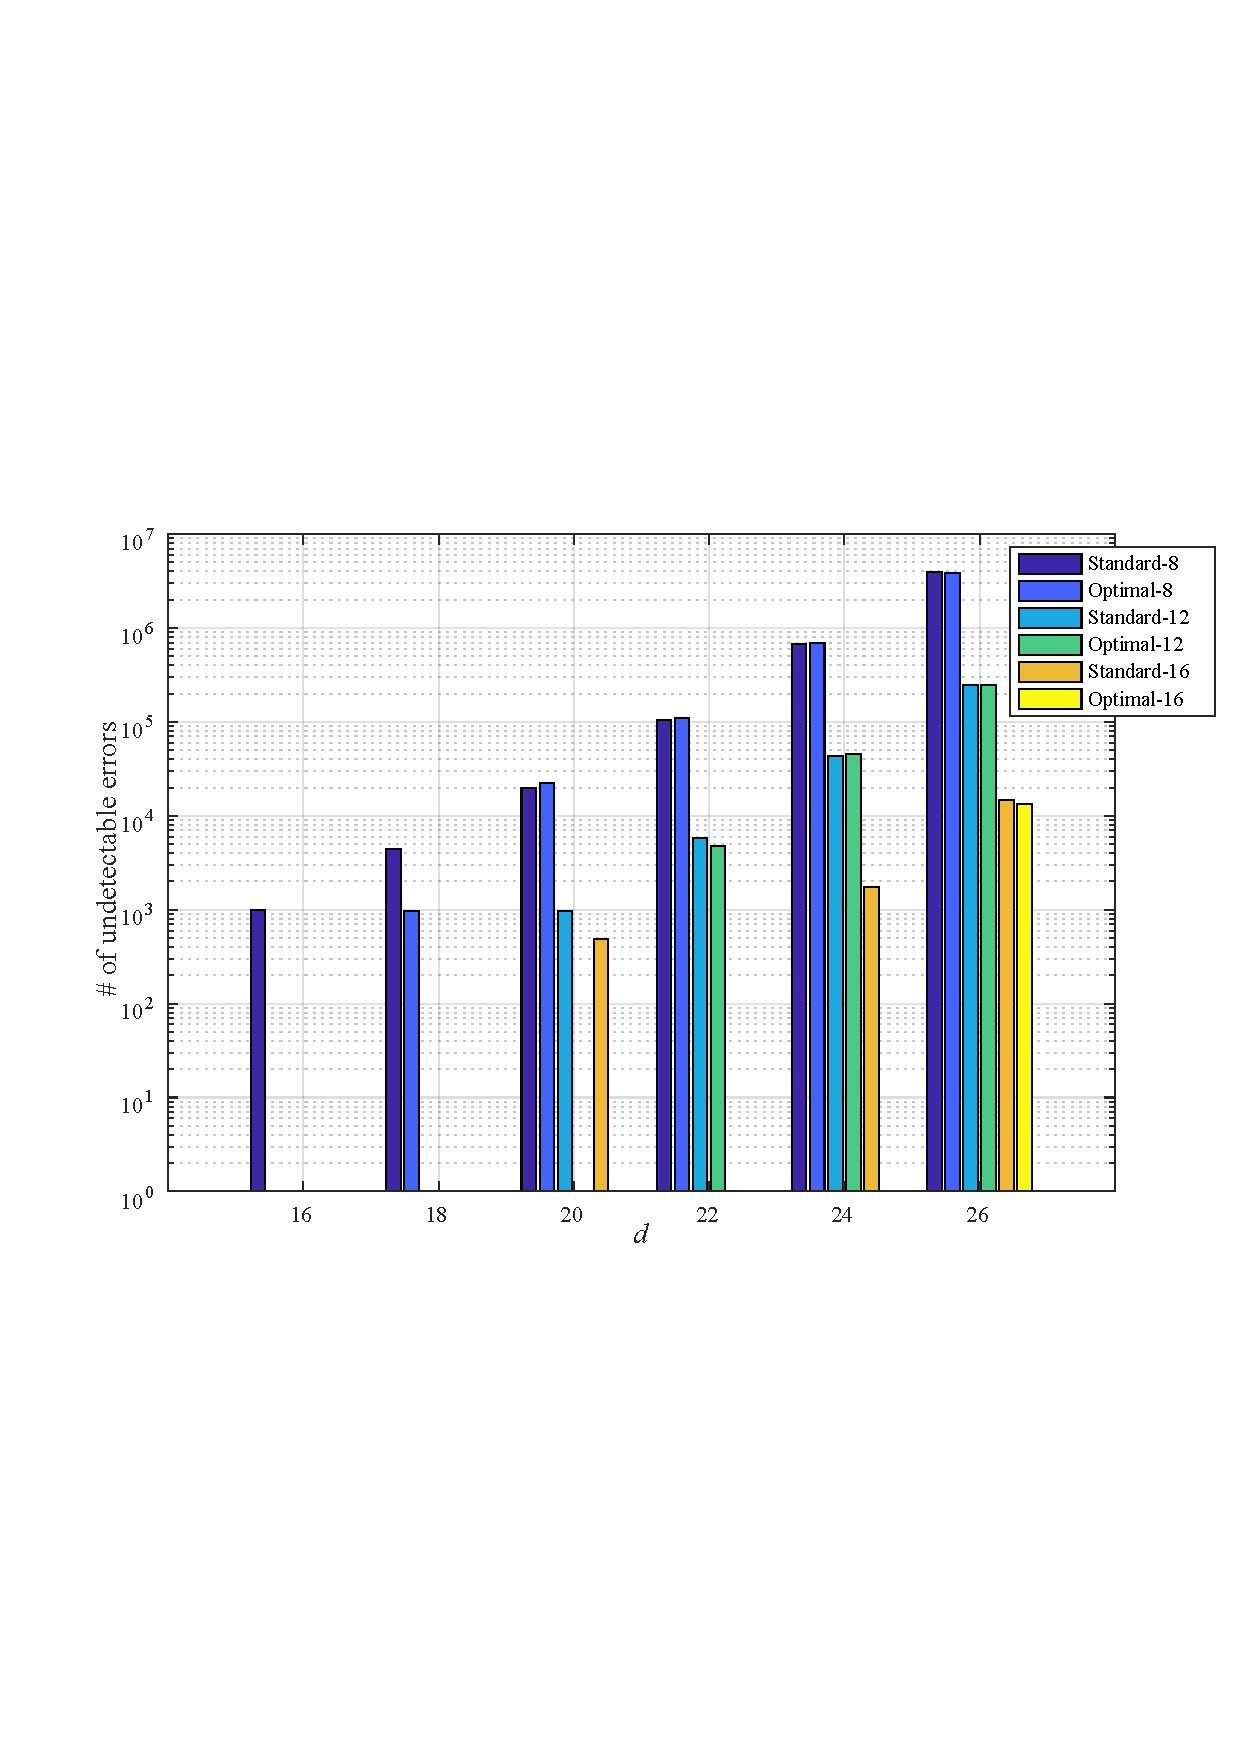
\includegraphics{Figures/spectrum_bar.pdf}}
\caption{An example of figure insertion}
\label{example_fig}
\end{figure}

\subsection{Equations}
An example of equations is given as follows.
\begin{theorem}
Let $a$, $b$, $c$ denote the sides of a triangle, respectively. If $a\perp b$, the pythagoras theorem is given as follows.
\begin{align}
c^2 = a^2 + b^2
\end{align}
\end{theorem}

\subsection{Tables}
An example of tables is shown in Table \ref{example_table}.
\renewcommand\arraystretch{1.1}
\begin{table}[h]
\center
\caption{Standard CRC Codes versus Optimal CRC Codes for Convolutional Code $G=(561~753)$ with $n=504$ Bits}
\scalebox{0.9}{
\begin{tabular}{r|c|c|cccccc}
\hline
\multirow{2}{*}{Name} & \multirow{2}{*}{Gen. Poly.} & \multicolumn{7}{c}{Undetected Error Distance Spectrum} \\
\cline{3-9}
 & & $d$ & 16 & 18 & 20 & 22 & 24 & 26 \\\hline\hline
Standard-8 & \multicolumn{1}{l}{0x19B} & & 983 & 4387 & 19909 & 105000 & 672724 & 3972970\\
Optimal-8 & \multicolumn{1}{l}{0x19D} & & 0 & 979 & 22349 & 111304 & 686314 & 3830340\\\hline
Standard-12 & \multicolumn{1}{l}{0x180F} & & 0 & 0 & 969 & 5815 & 42893 & 245211 \\
Optimal-12 & \multicolumn{1}{l}{0x108B} & & 0 & 0 & 0 & 4793 & 45795 & 246729\\\hline
Standard-16 & \multicolumn{1}{l}{0x11021} & & 0 & 0 & 484 & 0 & 1765 & 14752\\
Optimal-16 & \multicolumn{1}{l}{0x1F8FD} & & 0 & 0 & 0 & 0 & 0 & 13240\\\hline
\end{tabular}}
\label{example_table}
\end{table}


\section{Facebook network}


\subsection{Structural properties of the facebook network}


\subsection{Personalized network}


\subsection{Core node’s personalized network}

There are 40 core nodes in the Facebook network, which is the nodes that have more than 200 neighbors i.e. the degree of the nodes is greater than 200. And the average degree of the core nodes is 279.
\subsubsection{Community structure of core node’s personalized network}

We aim to find the community structure and compute the modularity scores using Fast-Greedy, Edge-Betweenness, and Infomap community detection algorithms for each of some core nodes’ personalized network.

For Node ID 1, the community figures based on different algorithms are shown in Fig \ref{1_3_1_1}, Fig \ref{1_3_1_2} and Fig \ref{1_3_1_3}.
\begin{figure}[h]
\centering
\begin{minipage}[t]{0.48\textwidth}
\centering
\scalebox{1}{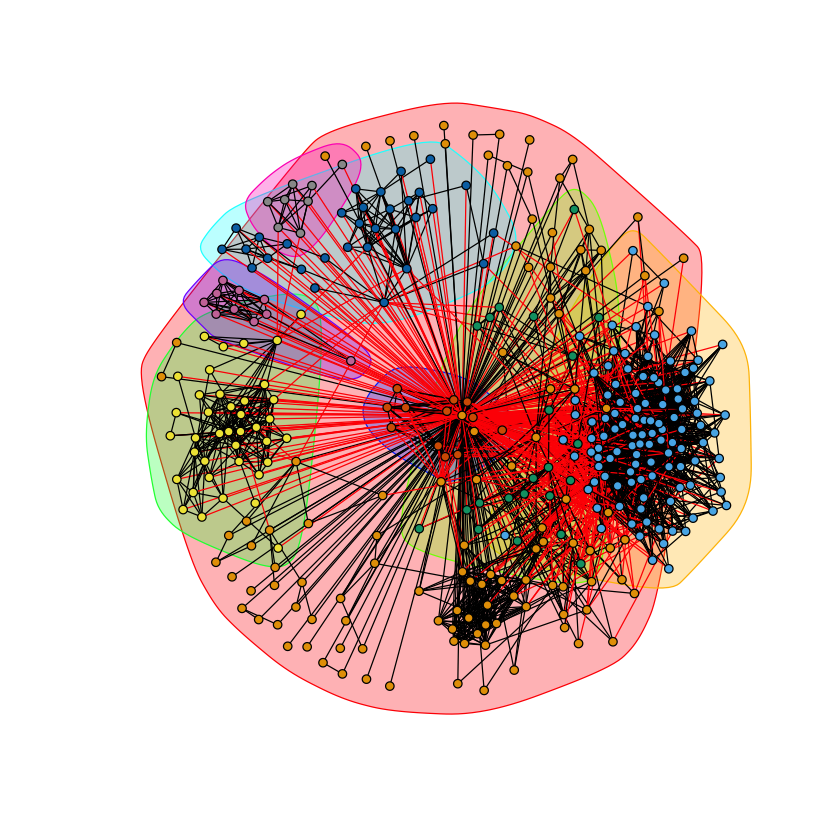
\includegraphics{Figures/1_3_1_1.png}}
\caption{community structure using Fast-Greedy algorithms}
\label{1_3_1_1}
\end{minipage}
\begin{minipage}[t]{0.48\textwidth}
\centering
\scalebox{1}{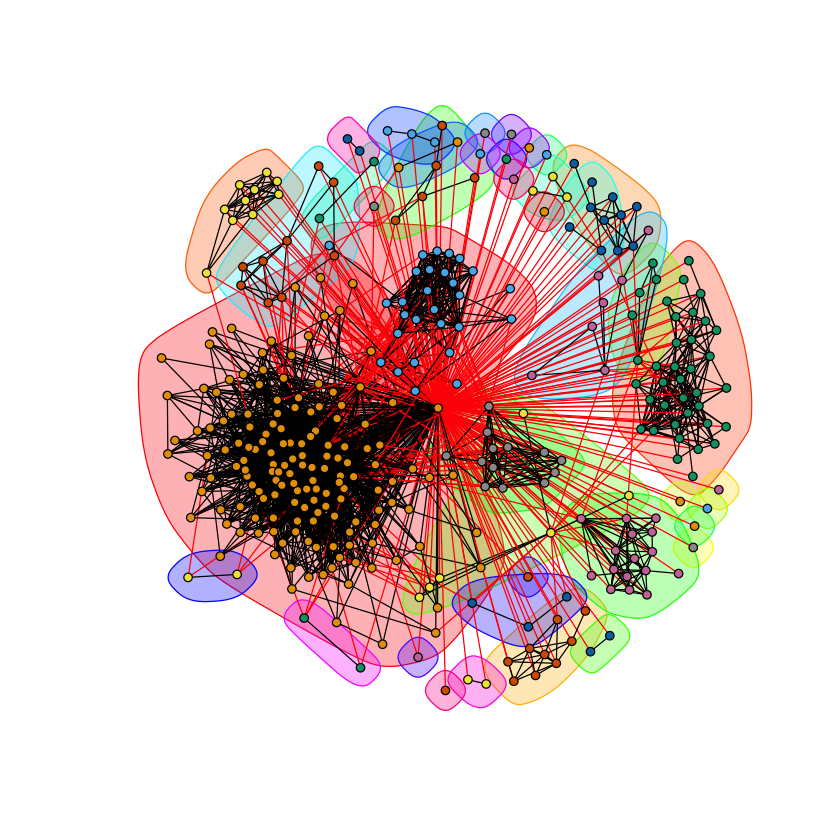
\includegraphics{Figures/1_3_1_2.png}}
\caption{community structure using Edge-Betweenness algorithms}
\label{1_3_1_2}
\end{minipage}
\end{figure}
\begin{figure}[h]
\centering
\scalebox{0.5}{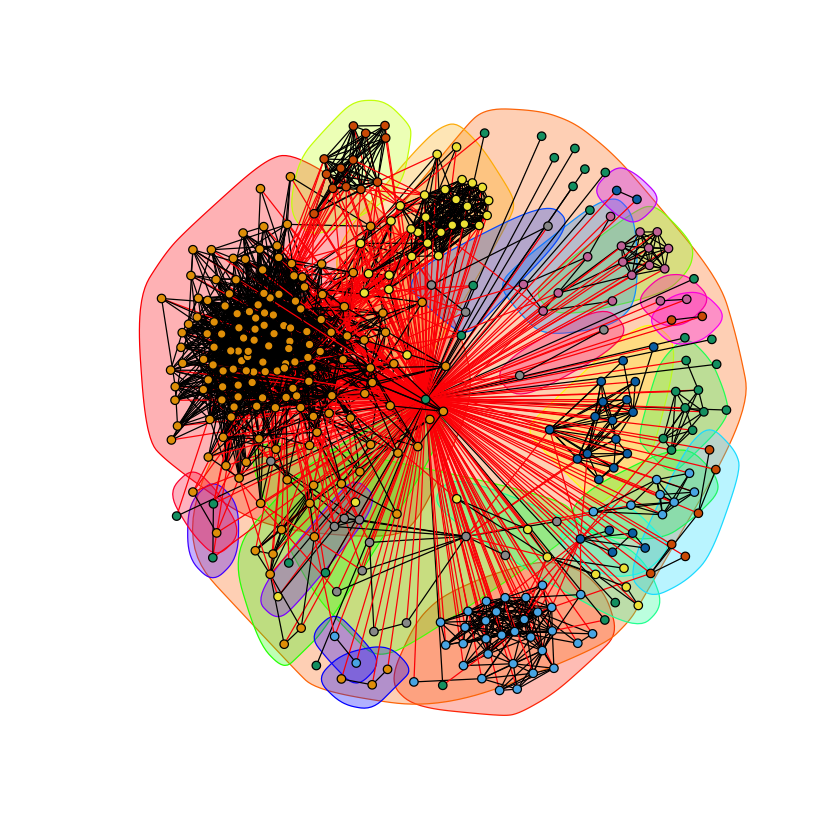
\includegraphics{Figures/1_3_1_3.png}}
\caption{community structure using Infomap algorithms}
\label{1_3_1_3}
\end{figure}

For Node ID 108, the community figures based on different algorithms are shown in Fig \ref{1_3_1_4}, Fig \ref{1_3_1_5} and Fig \ref{1_3_1_6}.
\begin{figure}[h]
\centering
\begin{minipage}[t]{0.48\textwidth}
\centering
\scalebox{1}{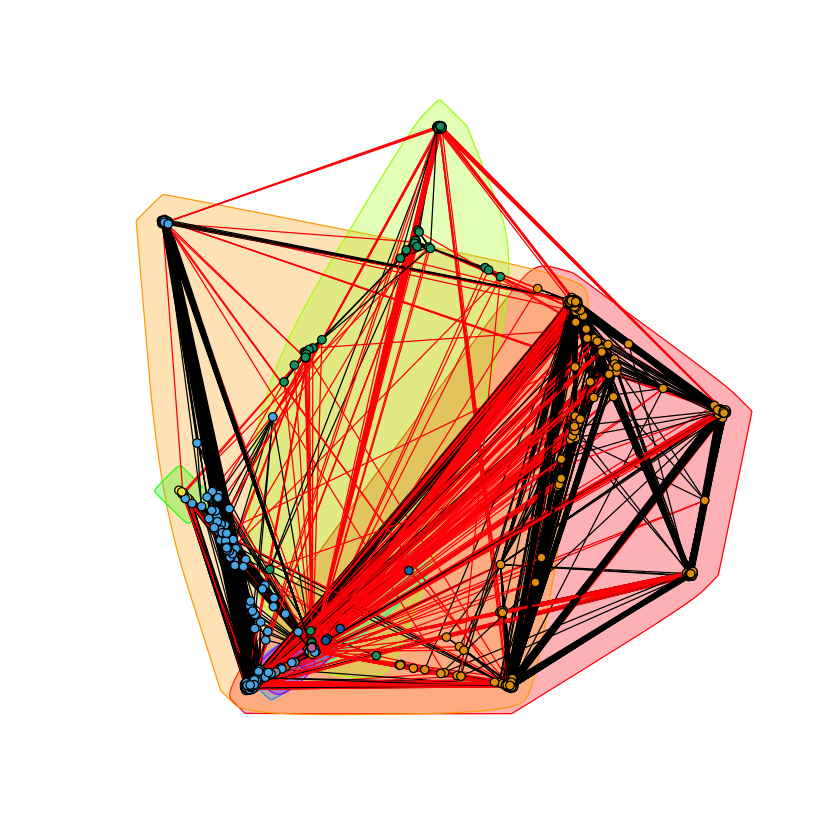
\includegraphics{Figures/1_3_1_4.png}}
\caption{community structure using Fast-Greedy algorithms}
\label{1_3_1_4}
\end{minipage}
\begin{minipage}[t]{0.48\textwidth}
\centering
\scalebox{1}{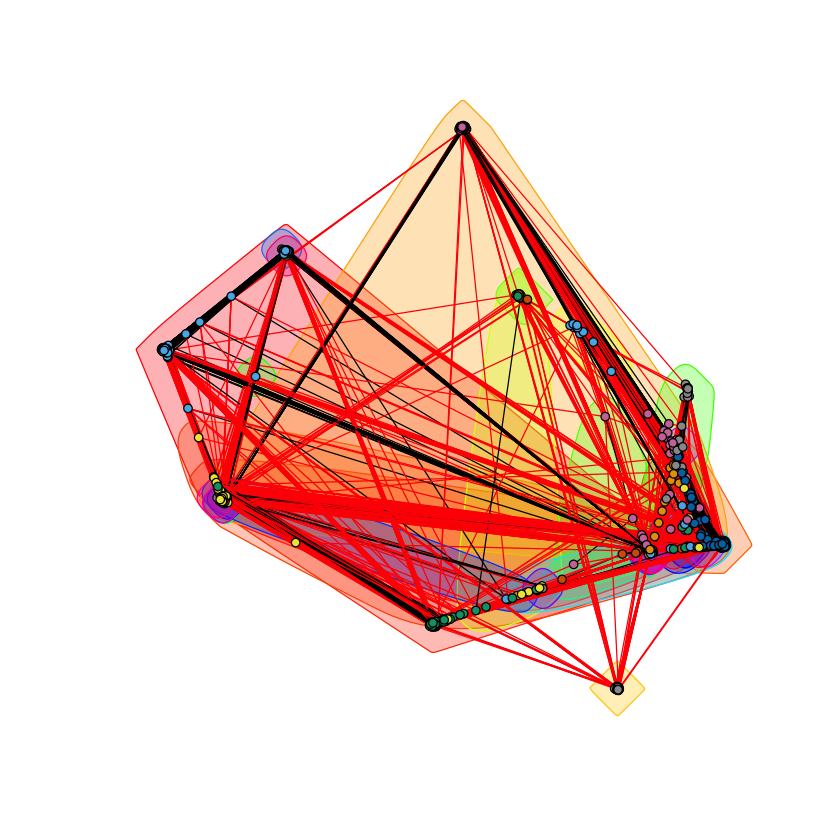
\includegraphics{Figures/1_3_1_5.png}}
\caption{community structure using Edge-Betweenness algorithms}
\label{1_3_1_5}
\end{minipage}
\end{figure}
\begin{figure}[h]
\centering
\scalebox{0.5}{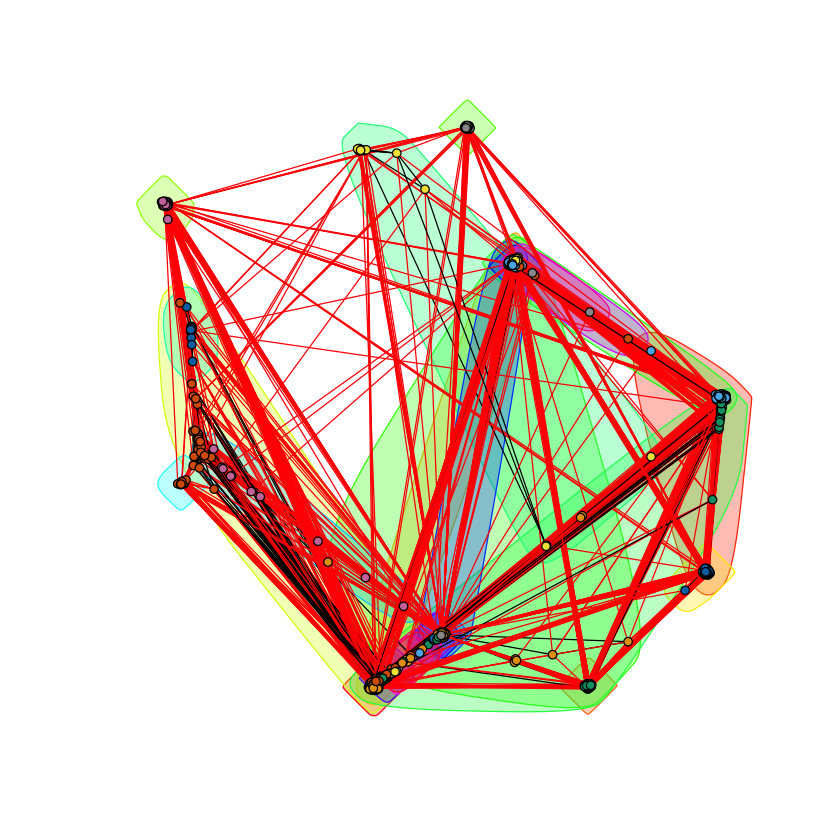
\includegraphics{Figures/1_3_1_6.png}}
\caption{community structure using Infomap algorithms}
\label{1_3_1_6}
\end{figure}

For Node ID 349, the community figures based on different algorithms are shown in Fig \ref{1_3_1_7}, Fig \ref{1_3_1_8} and Fig \ref{1_3_1_9}.
\begin{figure}[h]
\centering
\begin{minipage}[t]{0.48\textwidth}
\centering
\scalebox{1}{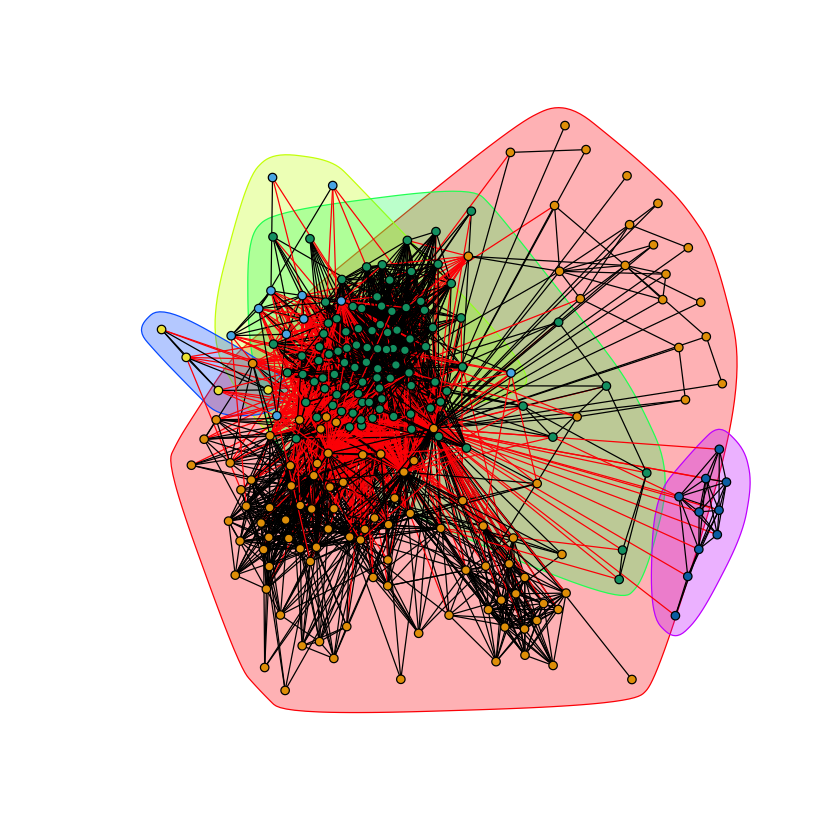
\includegraphics{Figures/1_3_1_7.png}}
\caption{community structure using Fast-Greedy algorithms}
\label{1_3_1_7}
\end{minipage}
\begin{minipage}[t]{0.48\textwidth}
\centering
\scalebox{1}{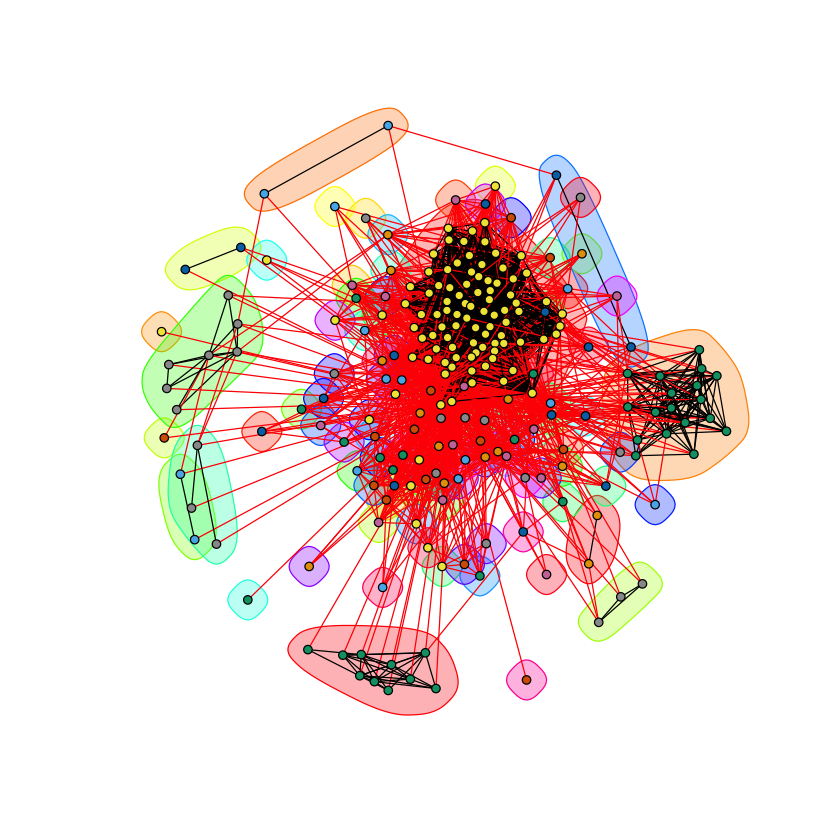
\includegraphics{Figures/1_3_1_8.png}}
\caption{community structure using Edge-Betweenness algorithms}
\label{1_3_1_8}
\end{minipage}
\end{figure}
\begin{figure}[h]
\centering
\scalebox{0.5}{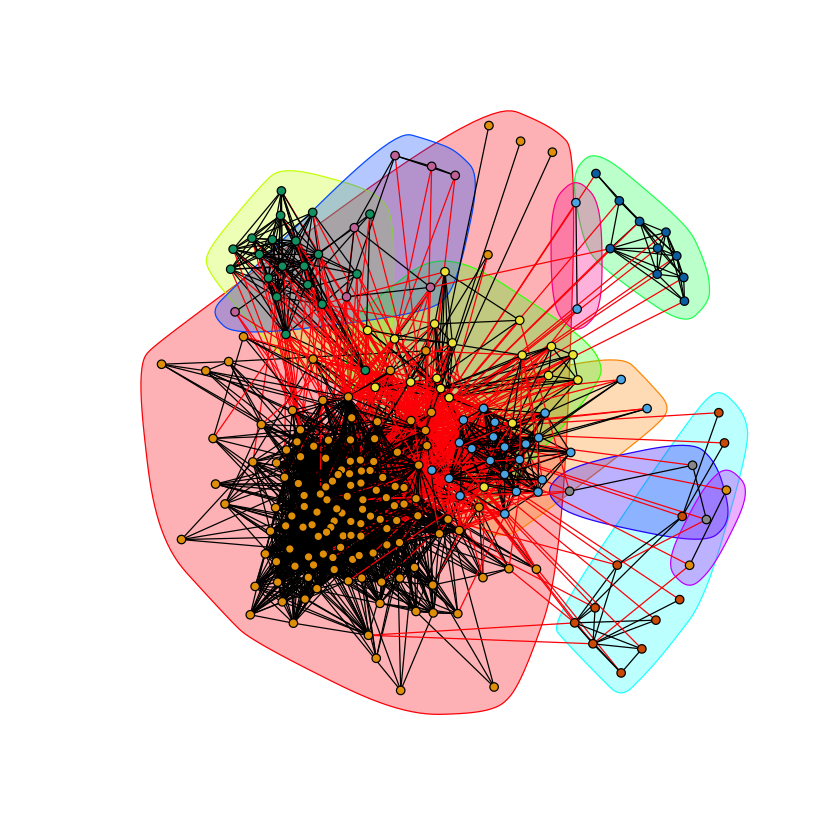
\includegraphics{Figures/1_3_1_9.png}}
\caption{community structure using Infomap algorithms}
\label{1_3_1_9}
\end{figure}

For Node ID 484, the community figures based on different algorithms are shown in Fig \ref{1_3_1_10}, Fig \ref{1_3_1_11} and Fig \ref{1_3_1_12}.
\begin{figure}[h]
\centering
\begin{minipage}[t]{0.48\textwidth}
\centering
\scalebox{1}{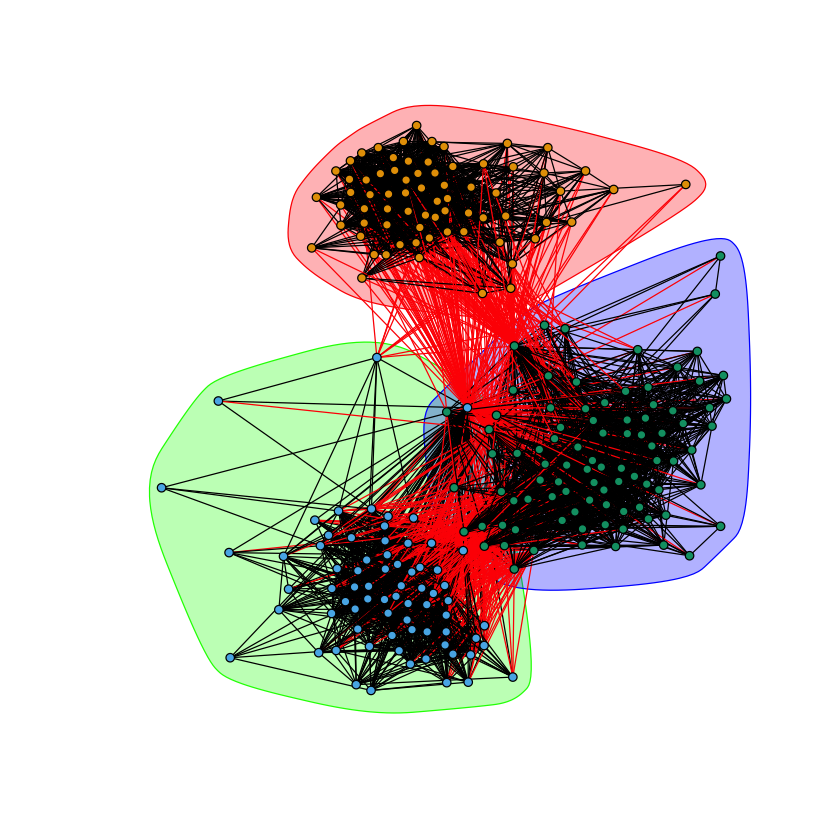
\includegraphics{Figures/1_3_1_10.png}}
\caption{community structure using Fast-Greedy algorithms}
\label{1_3_1_10}
\end{minipage}
\begin{minipage}[t]{0.48\textwidth}
\centering
\scalebox{1}{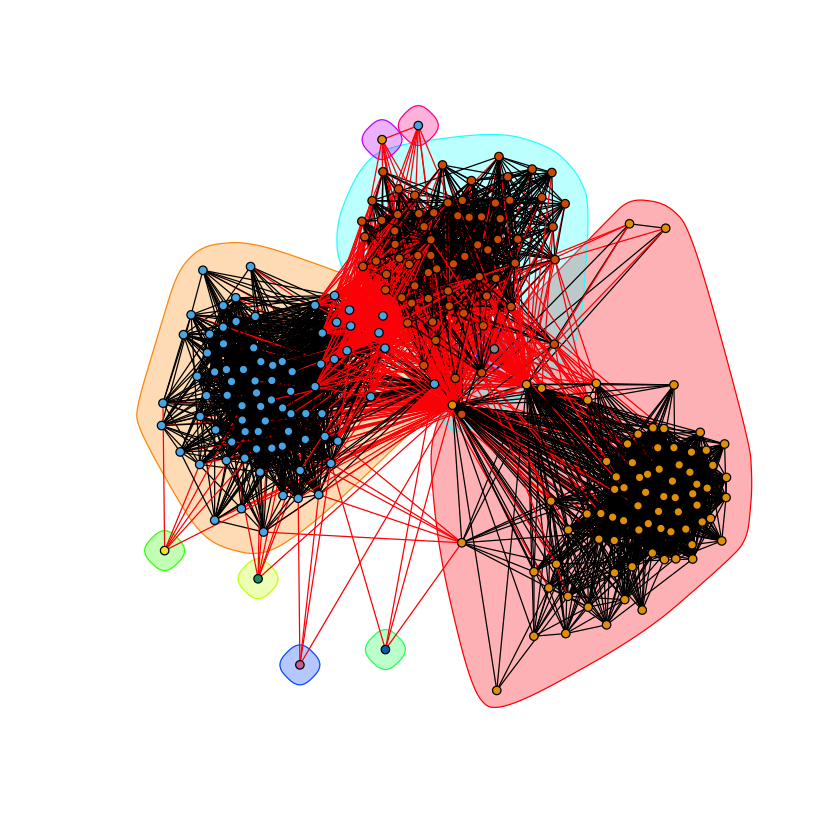
\includegraphics{Figures/1_3_1_11.png}}
\caption{community structure using Edge-Betweenness algorithms}
\label{1_3_1_11}
\end{minipage}
\end{figure}
\begin{figure}[h]
\centering
\scalebox{0.5}{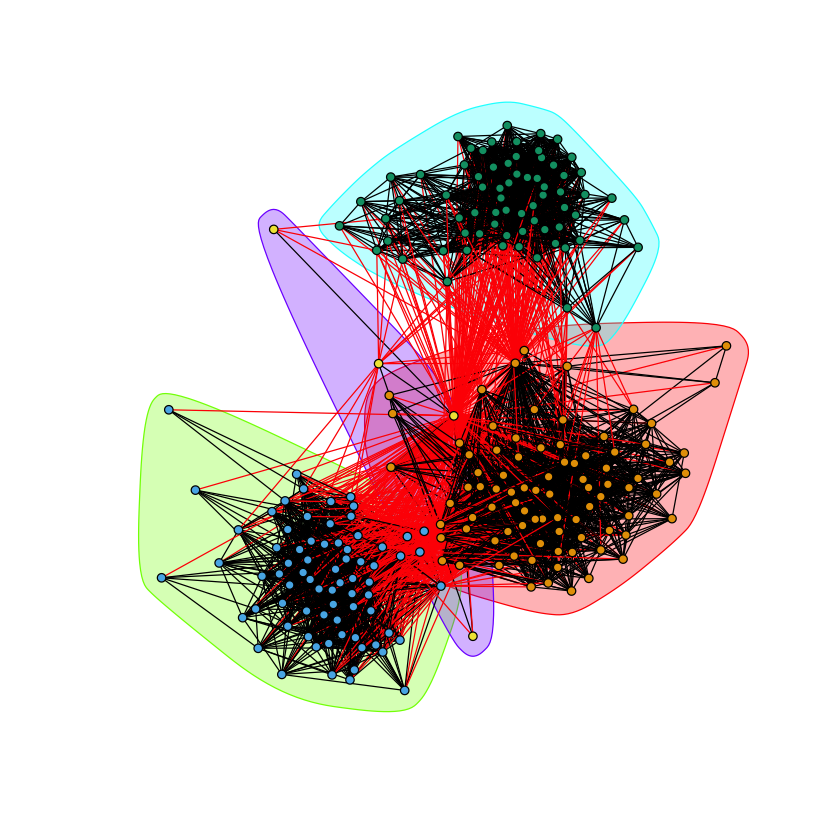
\includegraphics{Figures/1_3_1_12.png}}
\caption{community structure using Infomap algorithms}
\label{1_3_1_12}
\end{figure}

For Node ID 1087, the community figures based on different algorithms are shown in Fig \ref{1_3_1_13}, Fig \ref{1_3_1_14} and Fig \ref{1_3_1_15}.
\begin{figure}[h]
\centering
\begin{minipage}[t]{0.48\textwidth}
\centering
\scalebox{1}{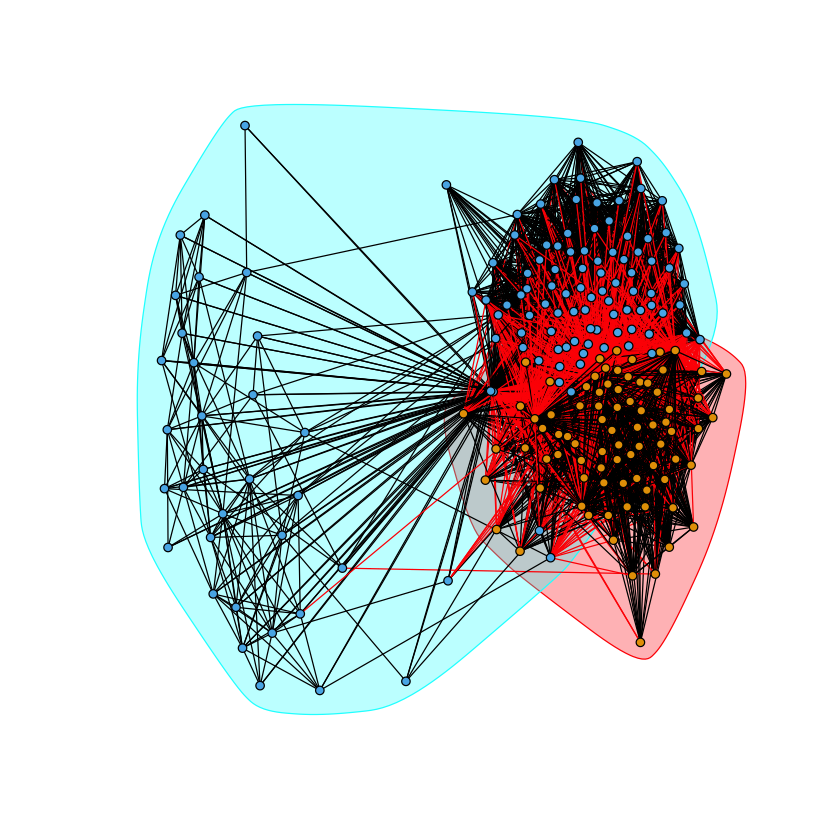
\includegraphics{Figures/1_3_1_13.png}}
\caption{community structure using Fast-Greedy algorithms}
\label{1_3_1_13}
\end{minipage}
\begin{minipage}[t]{0.48\textwidth}
\centering
\scalebox{1}{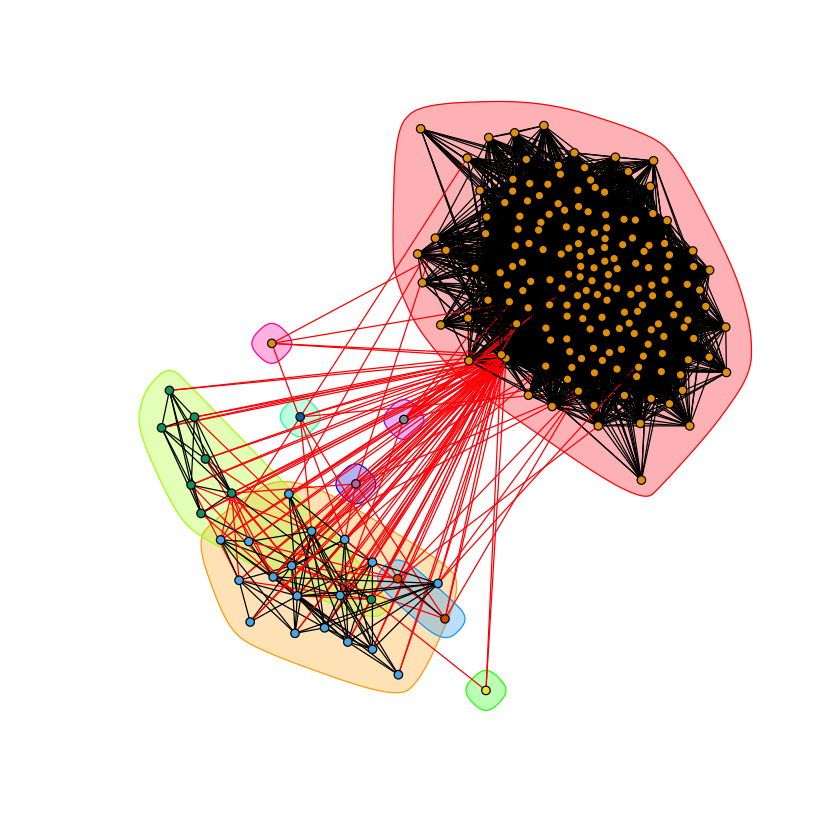
\includegraphics{Figures/1_3_1_14.png}}
\caption{community structure using Edge-Betweenness algorithms}
\label{1_3_1_14}
\end{minipage}
\end{figure}
\begin{figure}[h]
\centering
\scalebox{0.5}{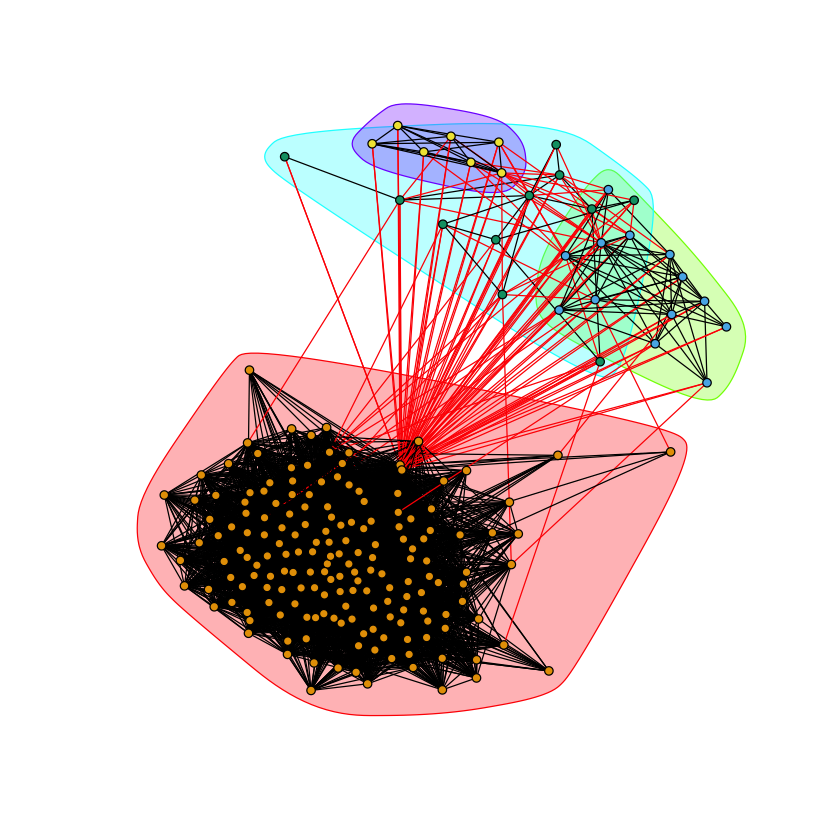
\includegraphics{Figures/1_3_1_15.png}}
\caption{community structure using Infomap algorithms}
\label{1_3_1_15}
\end{figure}

What's more, all the modularity scores from above core nodes' personalized network computed by different algorithms is shown in Table \ref{modtable}.

\begin{table}[h]
\center
\caption{The modularity scores for core nodes' personalized network}
\begin{tabular}{c|l|l|l} 
\textbf{Node ID} & \textbf{Fast-Greedy} & \textbf{Edge-Betweenness} & \textbf{Infomap}\\\hline
1 & 0.41310 & 0.35330 & 0.38912\\
108 & 0.43592 & - & 0.50842\\
349 & 0.25171 & 0.13352 & 0.20375\\
484 & 0.50700 & 0.48909 & 0.51527\\
1087 & 0.14553 & 0.02762 & 0.02690\\
\end{tabular}
\label{modtable}
\end{table}

\subsubsection{Community structure with the core node removed}

In this part, we aim to explore the effect on the community structure of a core node’s personalized network when the core node itself is removed from the personalized network.

For Node ID 1, the community figures based on different algorithms are shown in Fig \ref{1_3_2_1}, Fig \ref{1_3_2_2} and Fig \ref{1_3_2_3}.
\begin{figure}[h]
\centering
\begin{minipage}[t]{0.48\textwidth}
\centering
\scalebox{1}{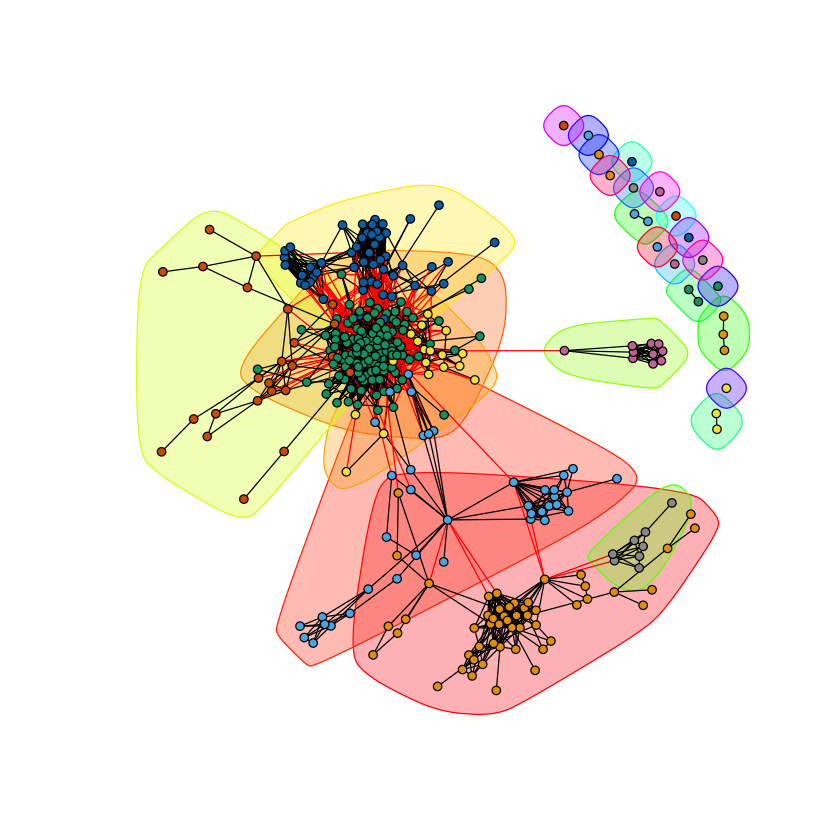
\includegraphics{Figures/1_3_2_1.png}}
\caption{community structure using Fast-Greedy algorithms}
\label{1_3_2_1}
\end{minipage}
\begin{minipage}[t]{0.48\textwidth}
\centering
\scalebox{1}{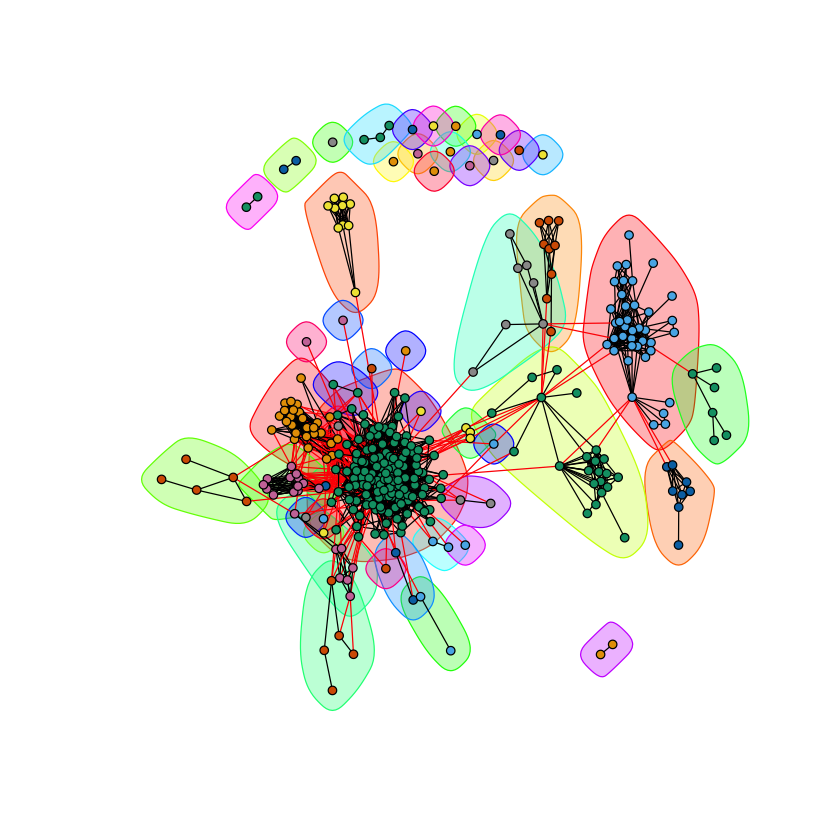
\includegraphics{Figures/1_3_2_2.png}}
\caption{community structure using Edge-Betweenness algorithms}
\label{1_3_2_2}
\end{minipage}
\end{figure}
\begin{figure}[h]
\centering
\scalebox{0.5}{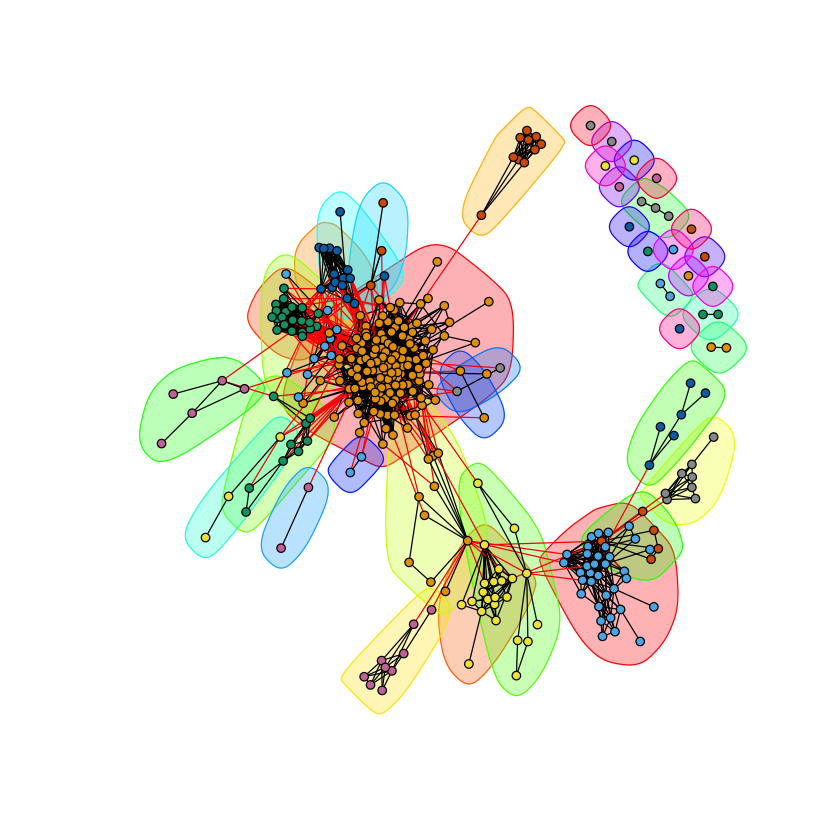
\includegraphics{Figures/1_3_2_3.png}}
\caption{community structure using Infomap algorithms}
\label{1_3_2_3}
\end{figure}

For Node ID 108, the community figures based on different algorithms are shown in Fig \ref{1_3_2_4}, Fig \ref{1_3_2_5} and Fig \ref{1_3_2_6}.
\begin{figure}[h]
\centering
\begin{minipage}[t]{0.48\textwidth}
\centering
\scalebox{1}{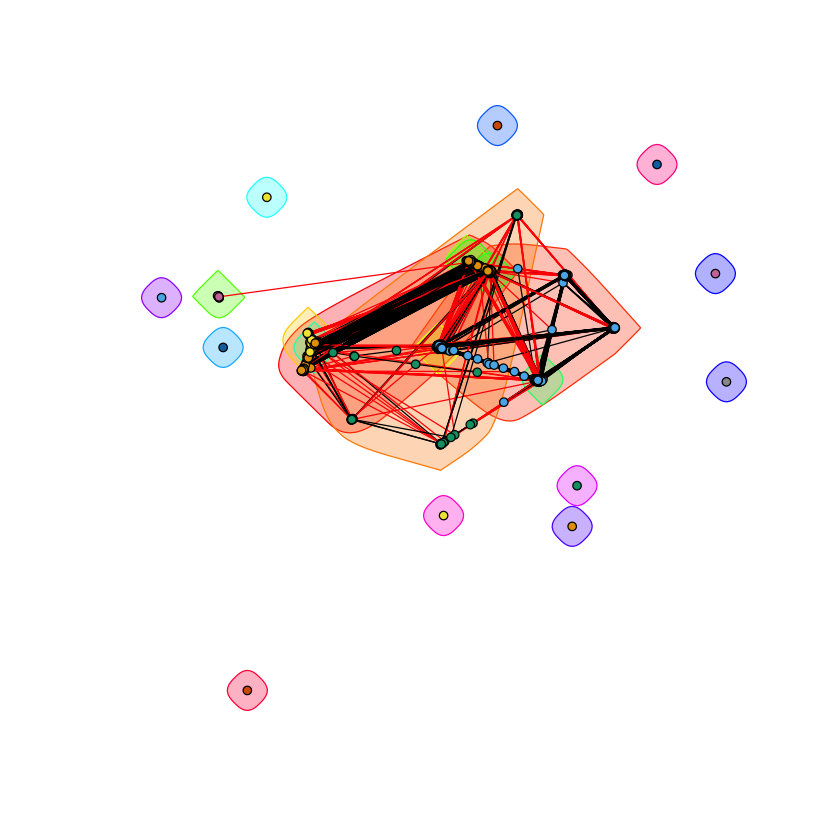
\includegraphics{Figures/1_3_2_4.png}}
\caption{community structure using Fast-Greedy algorithms}
\label{1_3_2_4}
\end{minipage}
\begin{minipage}[t]{0.48\textwidth}
\centering
\scalebox{1}{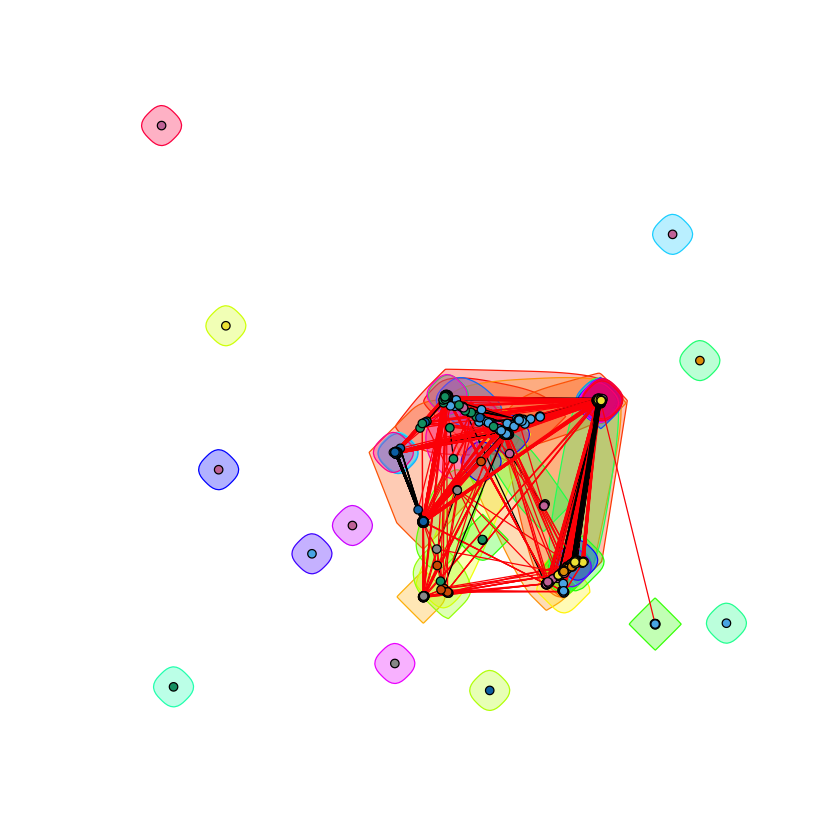
\includegraphics{Figures/1_3_2_5.png}}
\caption{community structure using Edge-Betweenness algorithms}
\label{1_3_2_5}
\end{minipage}
\end{figure}
\begin{figure}[h]
\centering
\scalebox{0.5}{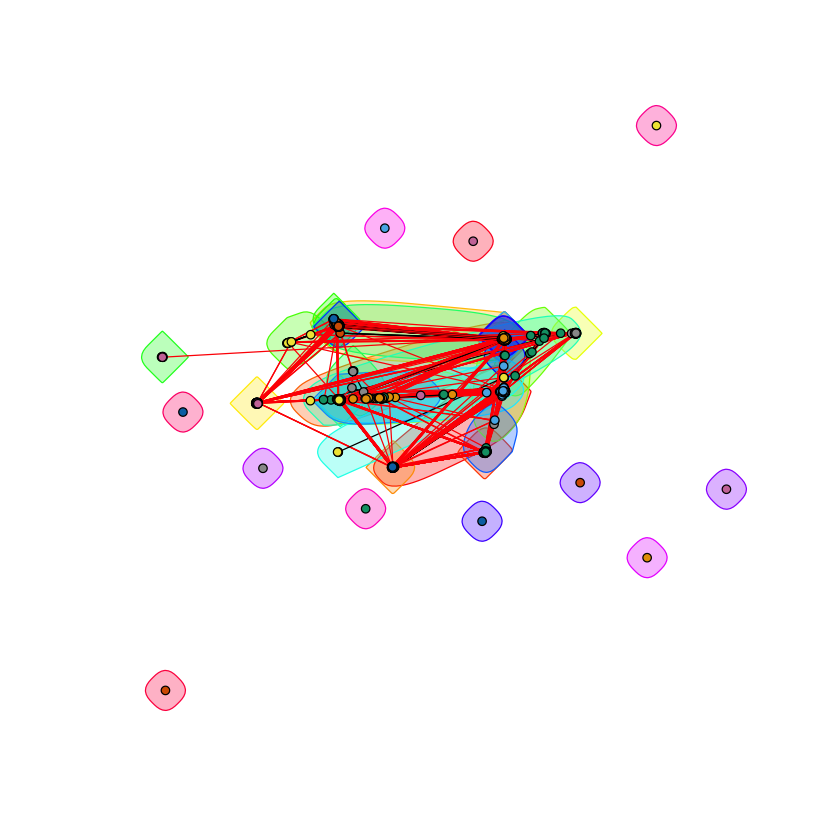
\includegraphics{Figures/1_3_2_6.png}}
\caption{community structure using Infomap algorithms}
\label{1_3_2_6}
\end{figure}

For Node ID 349, the community figures based on different algorithms are shown in Fig \ref{1_3_2_7}, Fig \ref{1_3_2_8} and Fig \ref{1_3_2_9}.
\begin{figure}[h]
\centering
\begin{minipage}[t]{0.48\textwidth}
\centering
\scalebox{1}{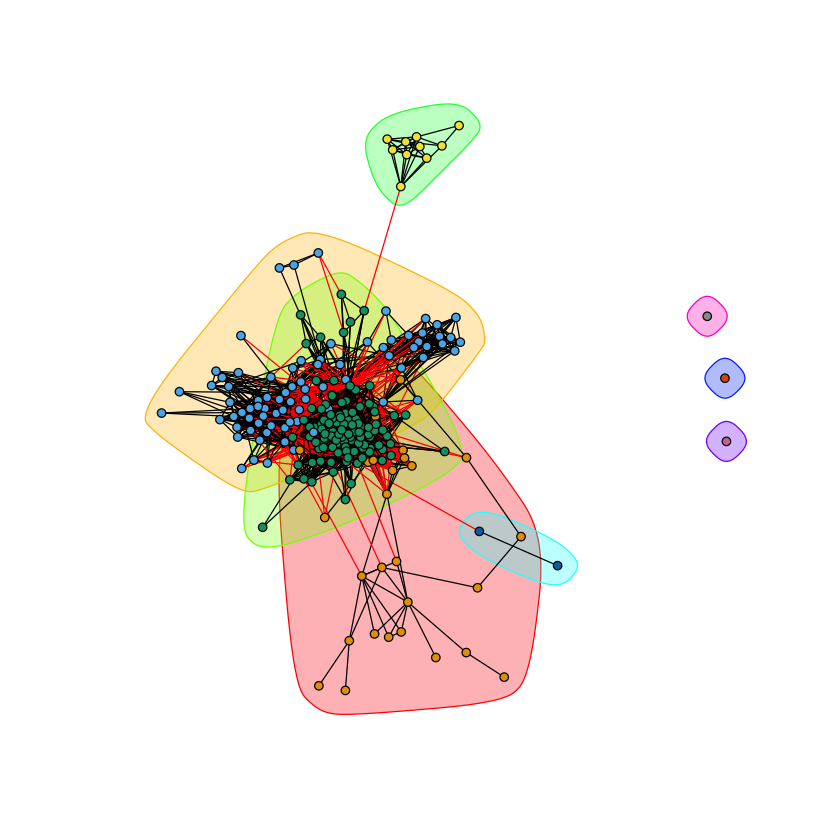
\includegraphics{Figures/1_3_2_7.png}}
\caption{community structure using Fast-Greedy algorithms}
\label{1_3_2_7}
\end{minipage}
\begin{minipage}[t]{0.48\textwidth}
\centering
\scalebox{1}{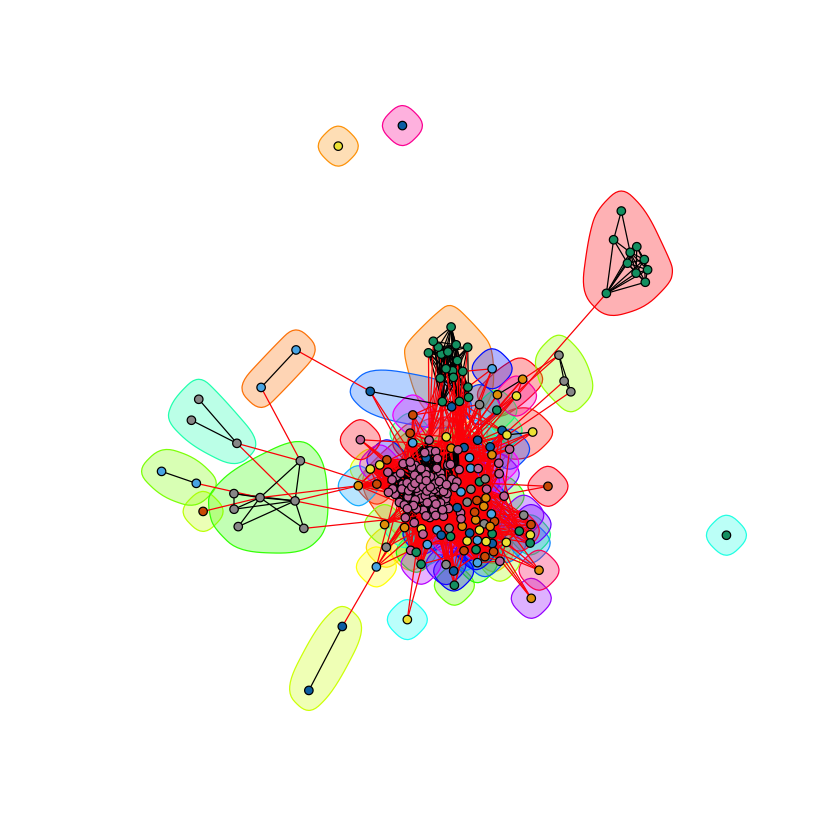
\includegraphics{Figures/1_3_2_8.png}}
\caption{community structure using Edge-Betweenness algorithms}
\label{1_3_2_8}
\end{minipage}
\end{figure}
\begin{figure}[h]
\centering
\scalebox{0.5}{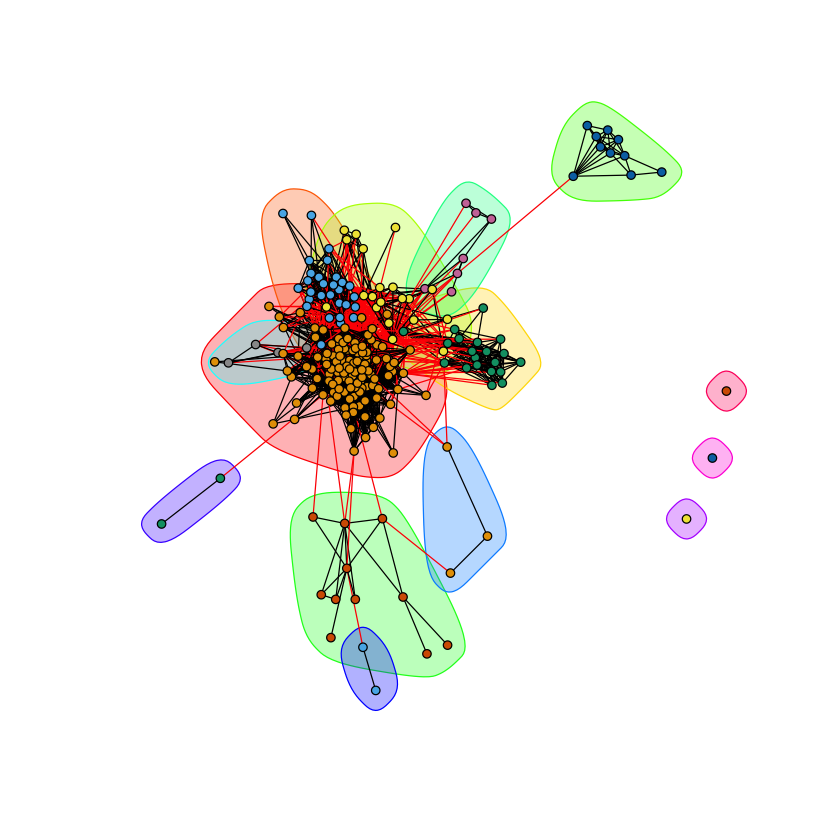
\includegraphics{Figures/1_3_2_9.png}}
\caption{community structure using Infomap algorithms}
\label{1_3_2_9}
\end{figure}

For Node ID 484, the community figures based on different algorithms are shown in Fig \ref{1_3_2_10}, Fig \ref{1_3_2_11} and Fig \ref{1_3_2_12}.
\begin{figure}[h]
\centering
\begin{minipage}[t]{0.48\textwidth}
\centering
\scalebox{1}{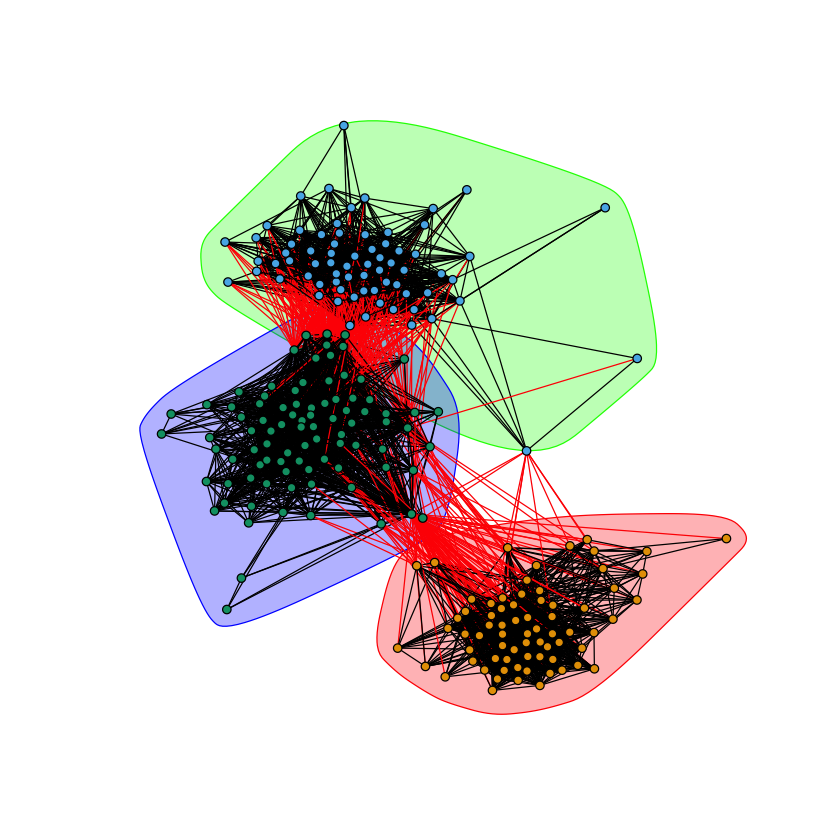
\includegraphics{Figures/1_3_2_10.png}}
\caption{community structure using Fast-Greedy algorithms}
\label{1_3_2_10}
\end{minipage}
\begin{minipage}[t]{0.48\textwidth}
\centering
\scalebox{1}{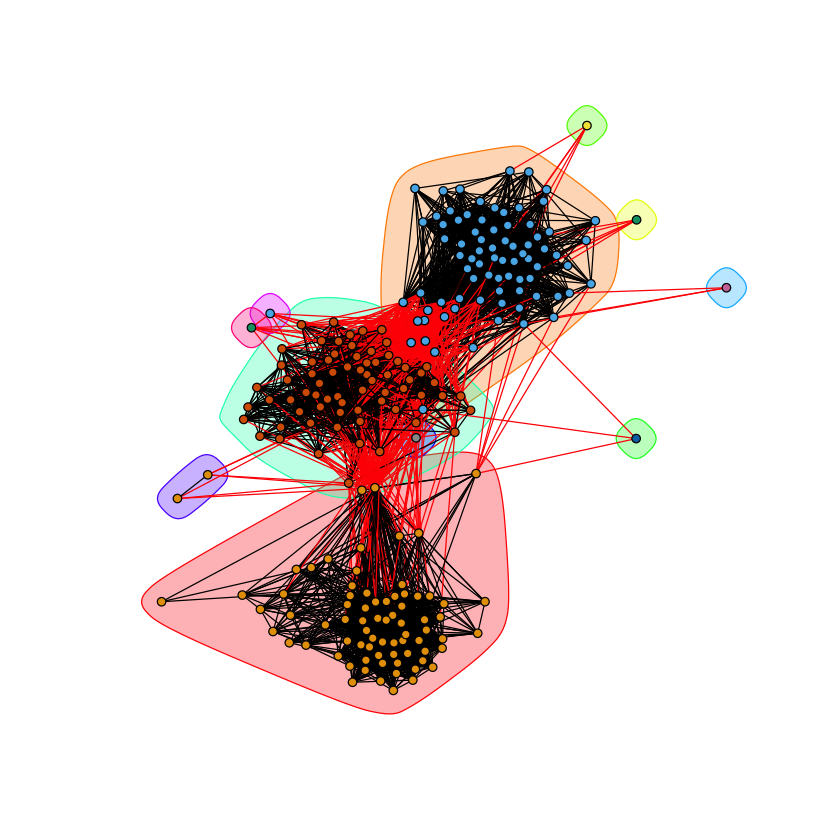
\includegraphics{Figures/1_3_2_11.png}}
\caption{community structure using Edge-Betweenness algorithms}
\label{1_3_2_11}
\end{minipage}
\end{figure}
\begin{figure}[h]
\centering
\scalebox{0.5}{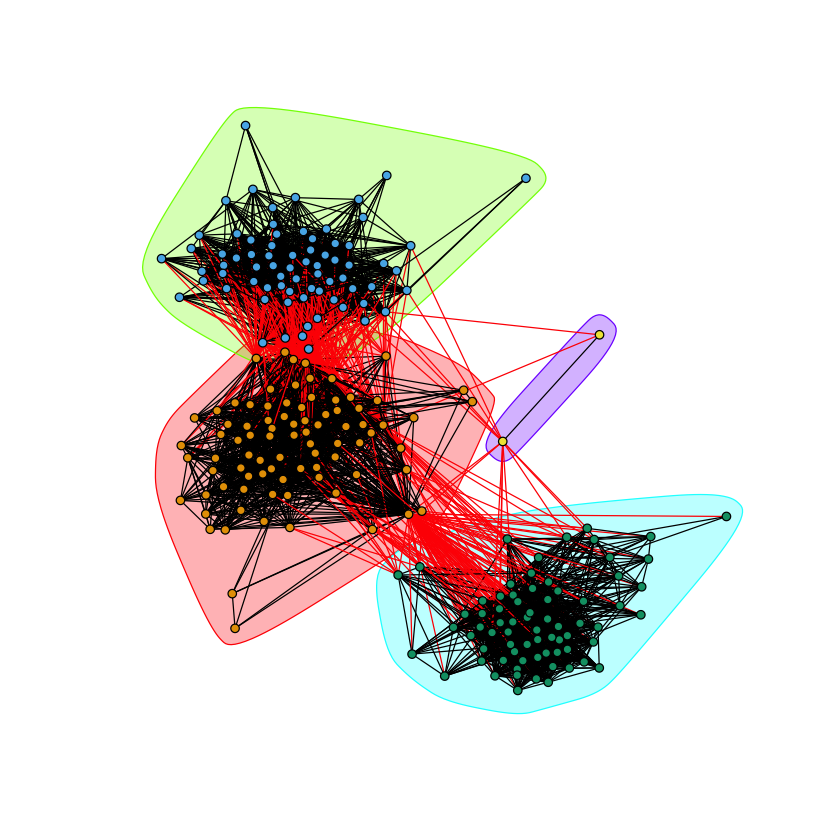
\includegraphics{Figures/1_3_2_12.png}}
\caption{community structure using Infomap algorithms}
\label{1_3_2_12}
\end{figure}

For Node ID 1087, the community figures based on different algorithms are shown in Fig \ref{1_3_2_13}, Fig \ref{1_3_2_14} and Fig \ref{1_3_2_15}.
\begin{figure}[h]
\centering
\begin{minipage}[t]{0.48\textwidth}
\centering
\scalebox{1}{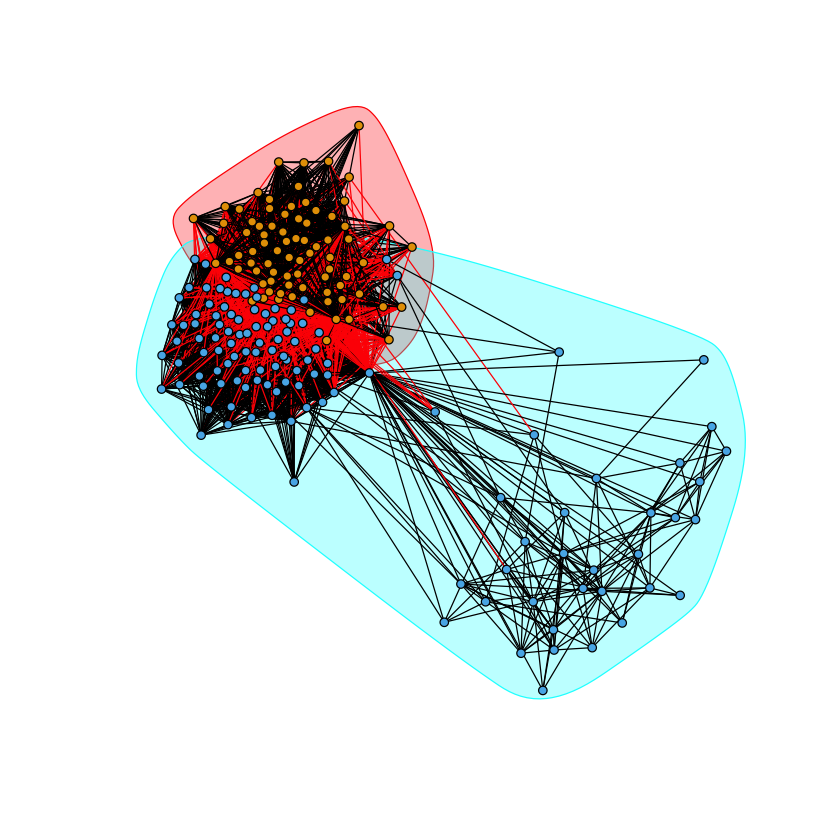
\includegraphics{Figures/1_3_2_13.png}}
\caption{community structure using Fast-Greedy algorithms}
\label{1_3_2_13}
\end{minipage}
\begin{minipage}[t]{0.48\textwidth}
\centering
\scalebox{1}{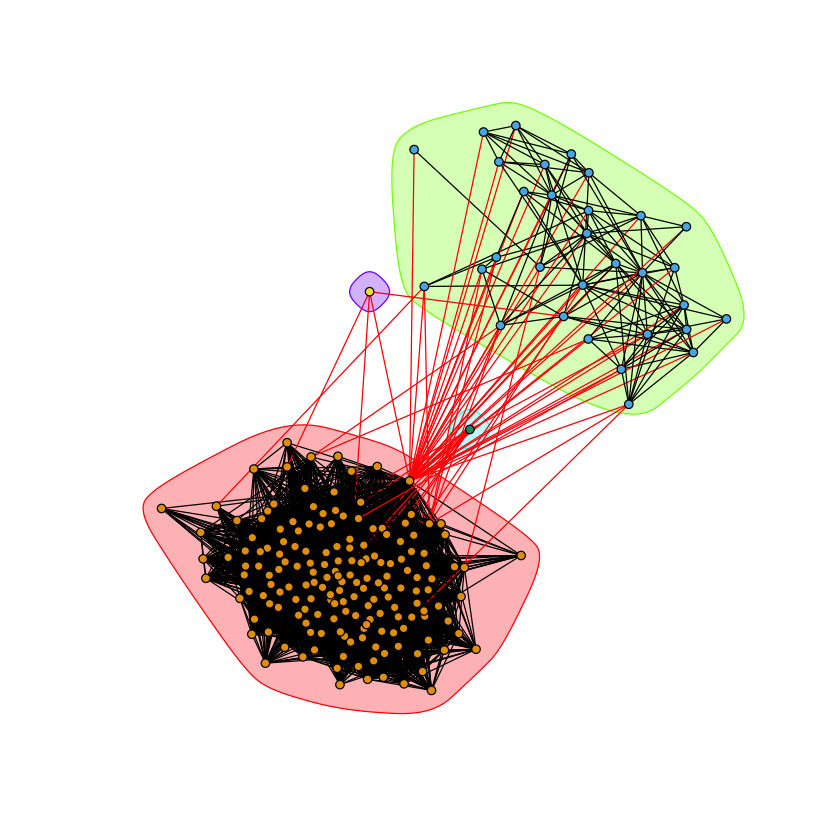
\includegraphics{Figures/1_3_2_14.png}}
\caption{community structure using Edge-Betweenness algorithms}
\label{1_3_2_14}
\end{minipage}
\end{figure}
\begin{figure}[h]
\centering
\scalebox{0.5}{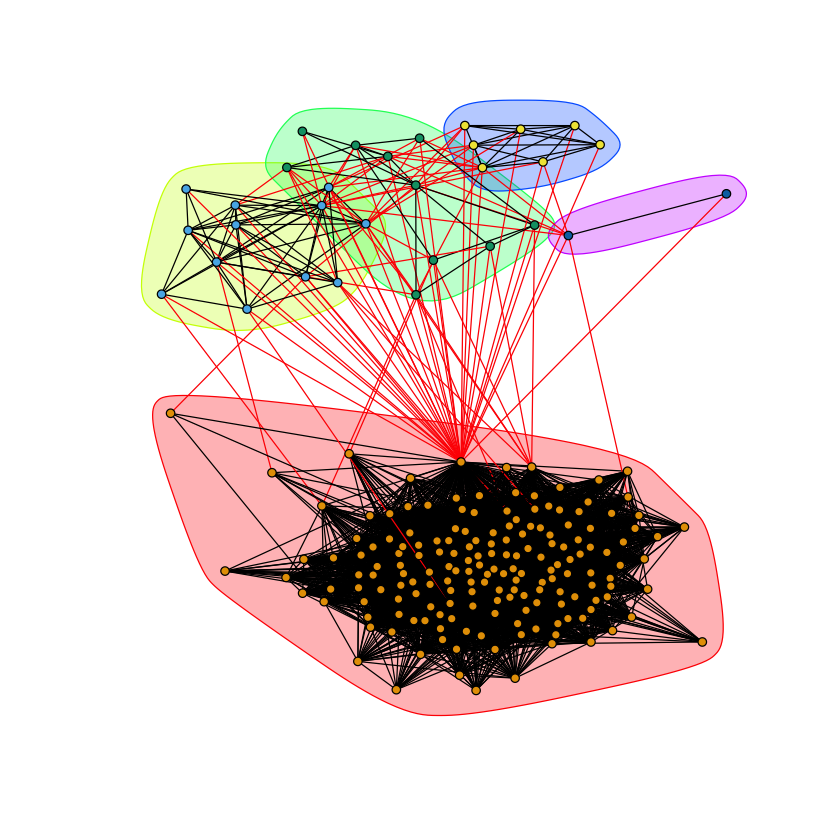
\includegraphics{Figures/1_3_2_15.png}}
\caption{community structure using Infomap algorithms}
\label{1_3_2_15}
\end{figure}

What's more, all the modularity scores from above core nodes' personalized network computed by different algorithms is shown in Table \ref{modtable2}.

\begin{table}[h]
\center
\caption{The modularity scores for core nodes' personalized network}
\begin{tabular}{c|l|l|l} 
\textbf{Node ID} & \textbf{Fast-Greedy} & \textbf{Edge-Betweenness} & \textbf{Infomap}\\\hline
1 & 0.41310 & 0.35330 & 0.38912\\
108 & 0.45812 & 0.52132 & 0.52068\\
349 & 0.24569 & 0.15056 & 0.24657\\
484 & 0.53421 & 0.51544 & 0.54344\\
1087 & 0.14819 & 0.03249 & 0.02737\\
\end{tabular}
\label{modtable2}
\end{table}

\subsubsection{Characteristic of nodes in the personalized network}

We aim to explore characteristics of nodes in the personalized network using two measures. These are two measures. One is embeddedness of a node that is defined as the number of mutual friends a node shares with the core node. Another that is dispersion of a node is defined as the sum of distances between every pair of the mutual friends the node shares with the core node. The distances should be calculated in a modified graph where the node (whose dispersion is being computed) and the core node are removed.

The expression relating the Embeddedness of a node to it’s degree is given as follows.
\begin{align}
Embedd(i) \leq Degree (i) - 1
\end{align}

For code code 1’s personalized network, the distribution of embeddedness and dispersion is shown in Fig \ref{1_3_3_1} and Fig \ref{1_3_3_2}.

\begin{figure}[h]
\centering
\begin{minipage}[t]{0.48\textwidth}
\centering
\scalebox{1}{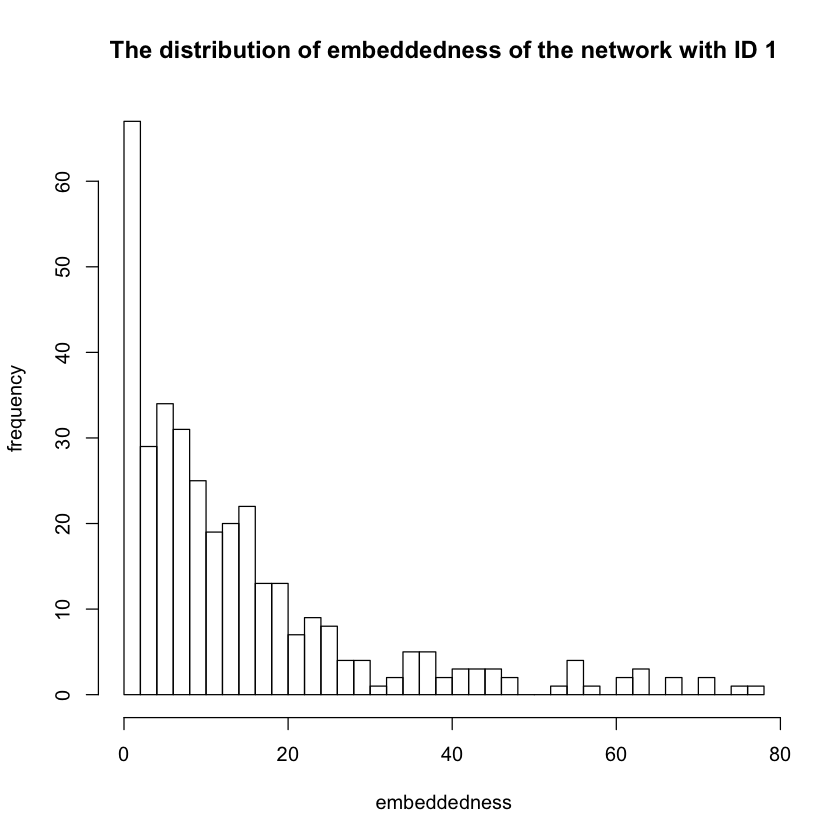
\includegraphics{Figures/1_3_3_1.png}}
\caption{The distribution of embeddedness}
\label{1_3_3_1}
\end{minipage}
\begin{minipage}[t]{0.48\textwidth}
\centering
\scalebox{1}{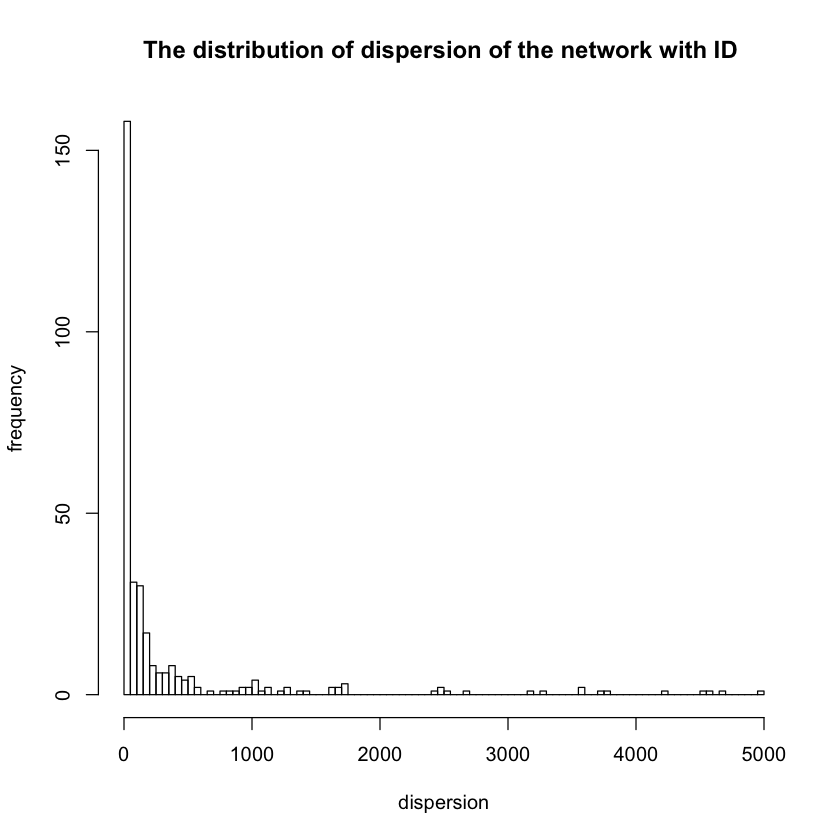
\includegraphics{Figures/1_3_3_2.png}}
\caption{The distribution of dispersion}
\label{1_3_3_2}
\end{minipage}
\end{figure}

For code code 108’s personalized network, the distribution of embeddedness and dispersion is shown in Fig \ref{1_3_3_3} and Fig \ref{1_3_3_4}.

\begin{figure}[h]
\centering
\begin{minipage}[t]{0.48\textwidth}
\centering
\scalebox{1}{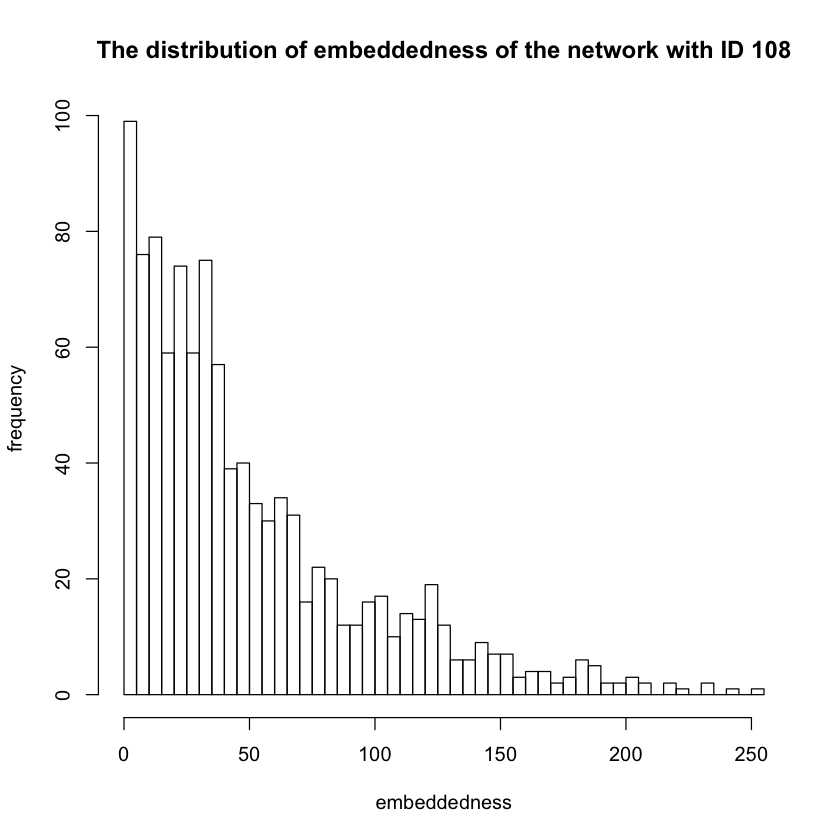
\includegraphics{Figures/1_3_3_3.png}}
\caption{The distribution of embeddedness}
\label{1_3_3_3}
\end{minipage}
\begin{minipage}[t]{0.48\textwidth}
\centering
\scalebox{1}{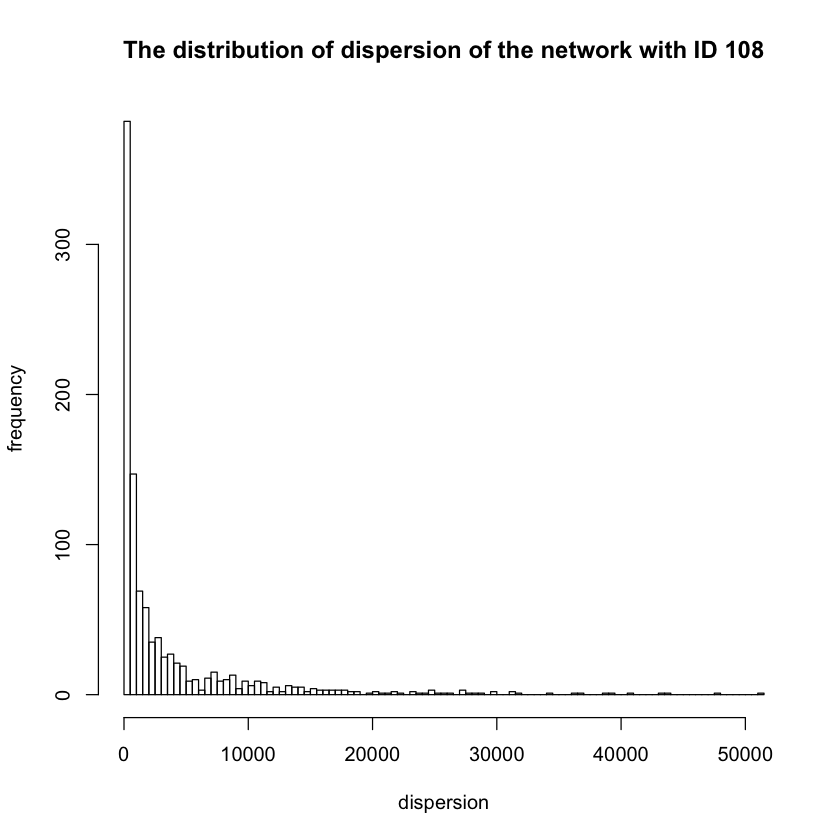
\includegraphics{Figures/1_3_3_4.png}}
\caption{The distribution of dispersion}
\label{1_3_3_4}
\end{minipage}
\end{figure}

For code code 349’s personalized network, the distribution of embeddedness and dispersion is shown in Fig \ref{1_3_3_5} and Fig \ref{1_3_3_6}.

\begin{figure}[h]
\centering
\begin{minipage}[t]{0.48\textwidth}
\centering
\scalebox{1}{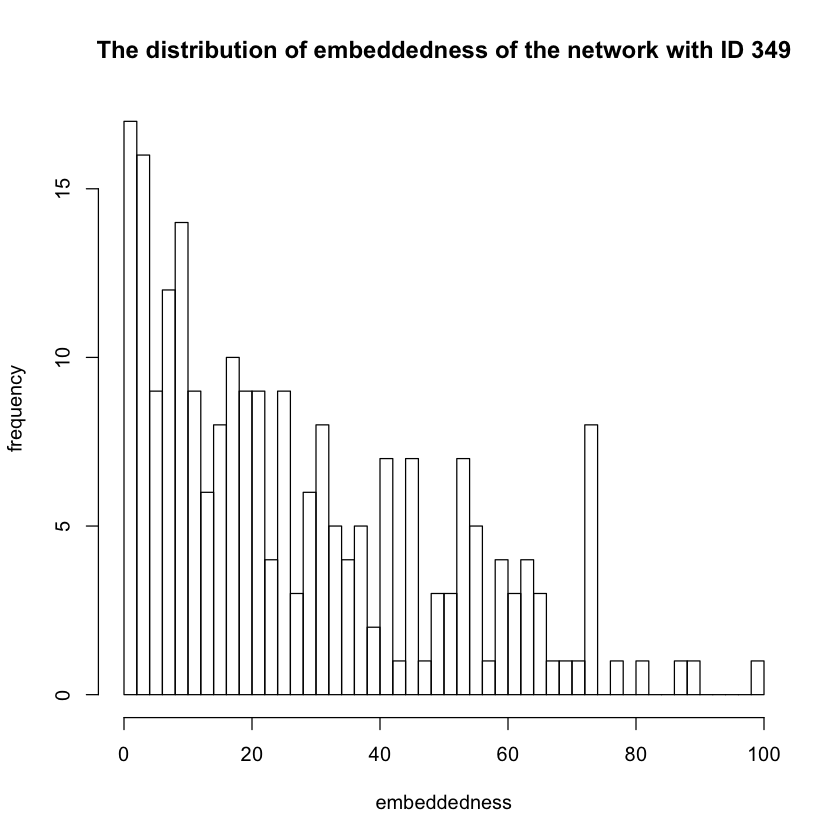
\includegraphics{Figures/1_3_3_5.png}}
\caption{The distribution of embeddedness}
\label{1_3_3_5}
\end{minipage}
\begin{minipage}[t]{0.48\textwidth}
\centering
\scalebox{1}{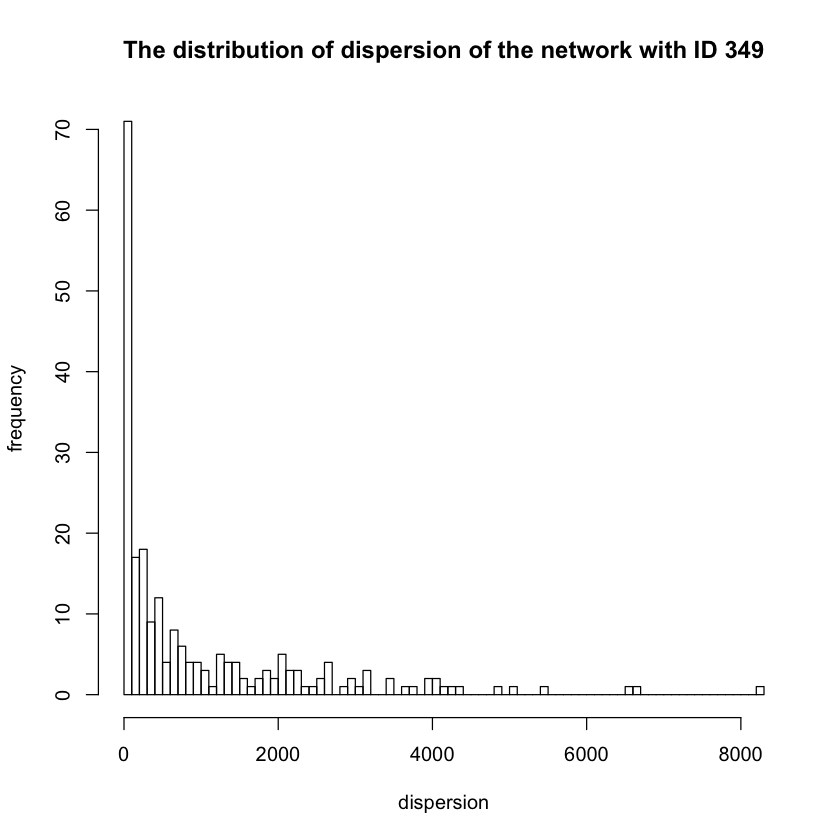
\includegraphics{Figures/1_3_3_6.png}}
\caption{The distribution of dispersion}
\label{1_3_3_6}
\end{minipage}
\end{figure}

For code code 484’s personalized network, the distribution of embeddedness and dispersion is shown in Fig \ref{1_3_3_7} and Fig \ref{1_3_3_8}.

\begin{figure}[h]
\centering
\begin{minipage}[t]{0.48\textwidth}
\centering
\scalebox{1}{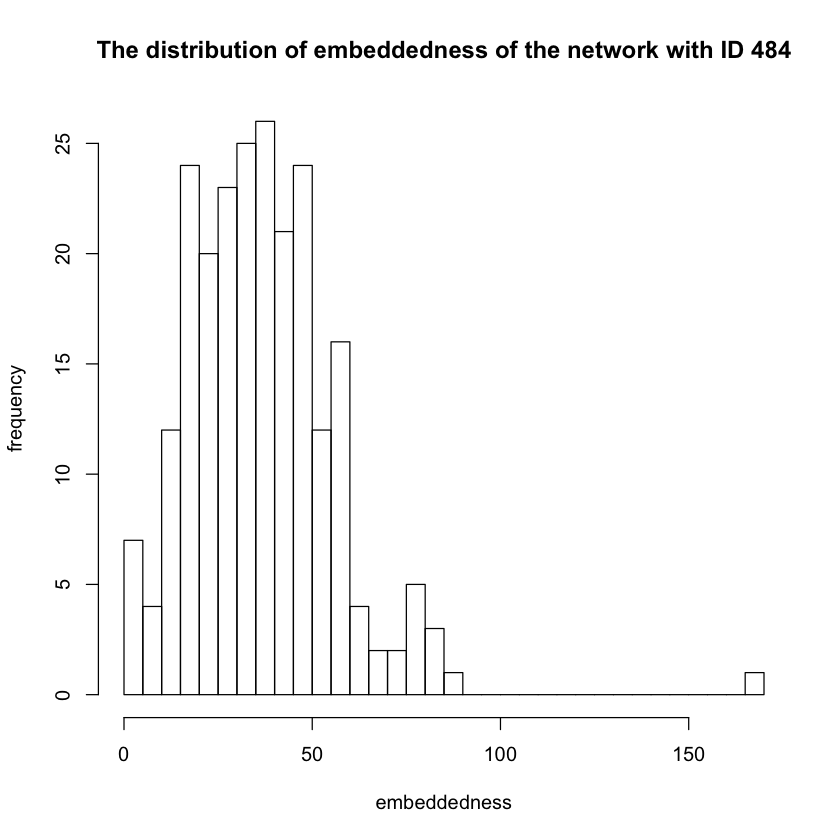
\includegraphics{Figures/1_3_3_7.png}}
\caption{The distribution of embeddedness}
\label{1_3_3_7}
\end{minipage}
\begin{minipage}[t]{0.48\textwidth}
\centering
\scalebox{1}{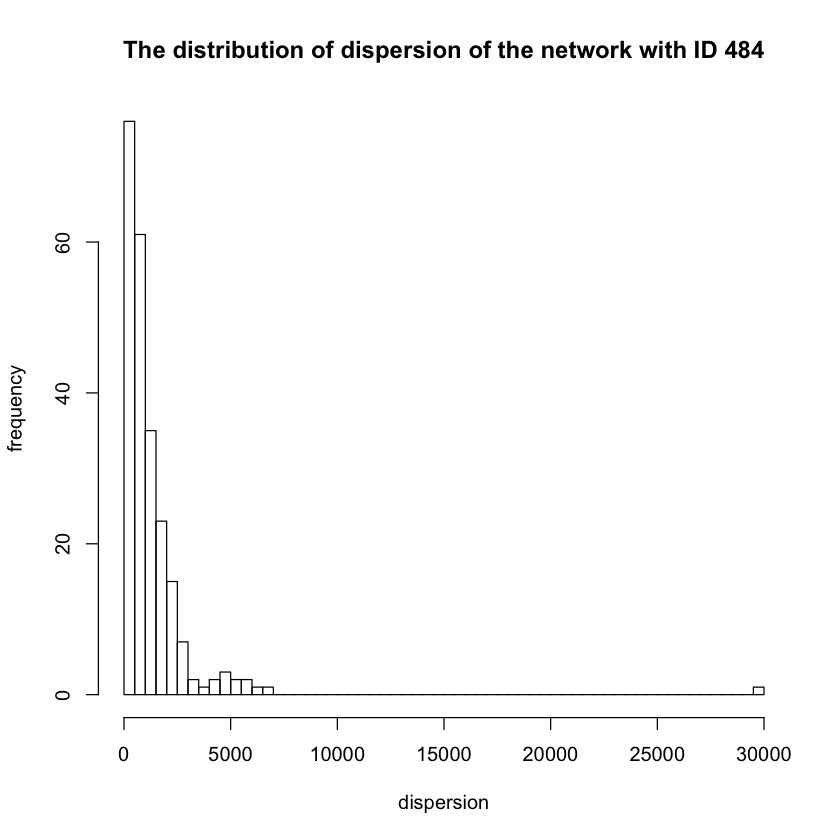
\includegraphics{Figures/1_3_3_8.png}}
\caption{The distribution of dispersion}
\label{1_3_3_8}
\end{minipage}
\end{figure}

For code code 1087’s personalized network, the distribution of embeddedness and dispersion is shown in Fig \ref{1_3_3_9} and Fig \ref{1_3_3_10}.

\begin{figure}[h]
\centering
\begin{minipage}[t]{0.48\textwidth}
\centering
\scalebox{1}{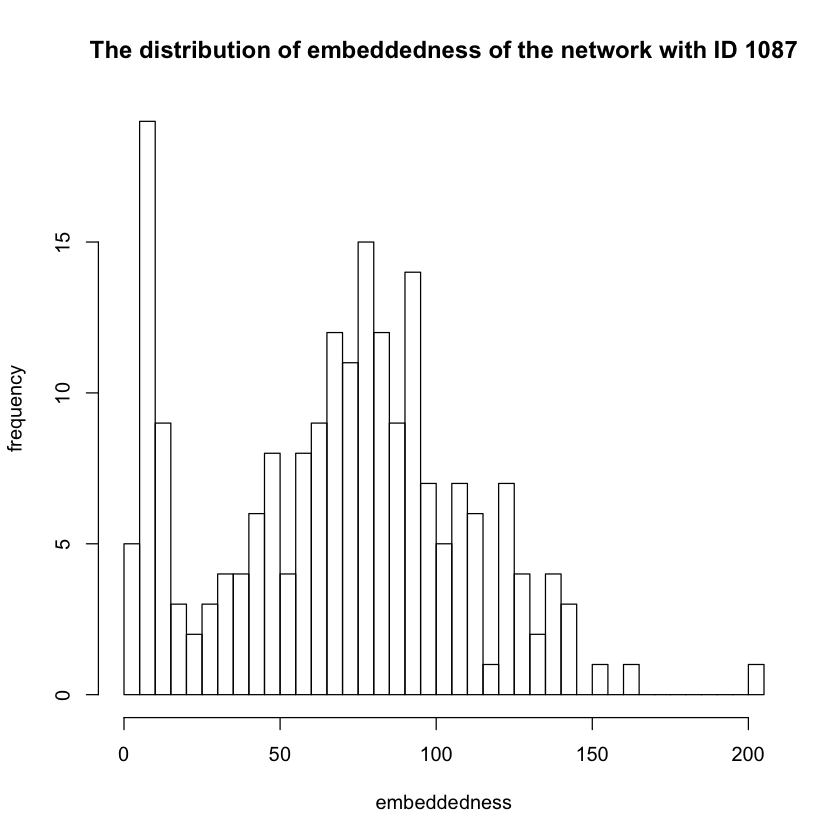
\includegraphics{Figures/1_3_3_9.png}}
\caption{The distribution of embeddedness}
\label{1_3_3_9}
\end{minipage}
\begin{minipage}[t]{0.48\textwidth}
\centering
\scalebox{1}{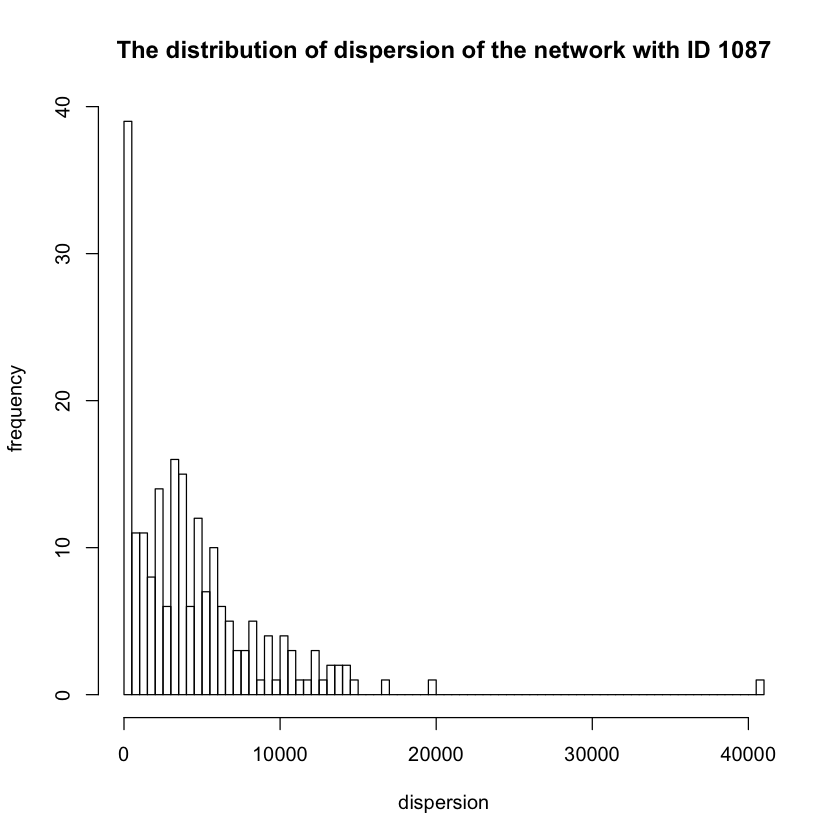
\includegraphics{Figures/1_3_3_10.png}}
\caption{The distribution of dispersion}
\label{1_3_3_10}
\end{minipage}
\end{figure}


For each of the core node’s personalized network, apply Fast-Greedy algorithm to detect the community structure of the personalized network and use colors and highlight the node with maximum dispersion and the edges incident to this node to plot this community.

For code code 1’s personalized network, the community structure is shown in Fig \ref{1_3_4_1}.
For code code 108’s personalized network, the community structure is shown in Fig \ref{1_3_4_2}.
For code code 349’s personalized network, the community structure is shown in Fig \ref{1_3_4_3}.
For code code 484’s personalized network, the community structure is shown in Fig \ref{1_3_4_4}.
For code code 1087’s personalized network, the community structure is shown in Fig \ref{1_3_4_5}.

\begin{figure}[h]
\centering
\begin{minipage}[t]{0.48\textwidth}
\centering
\scalebox{1}{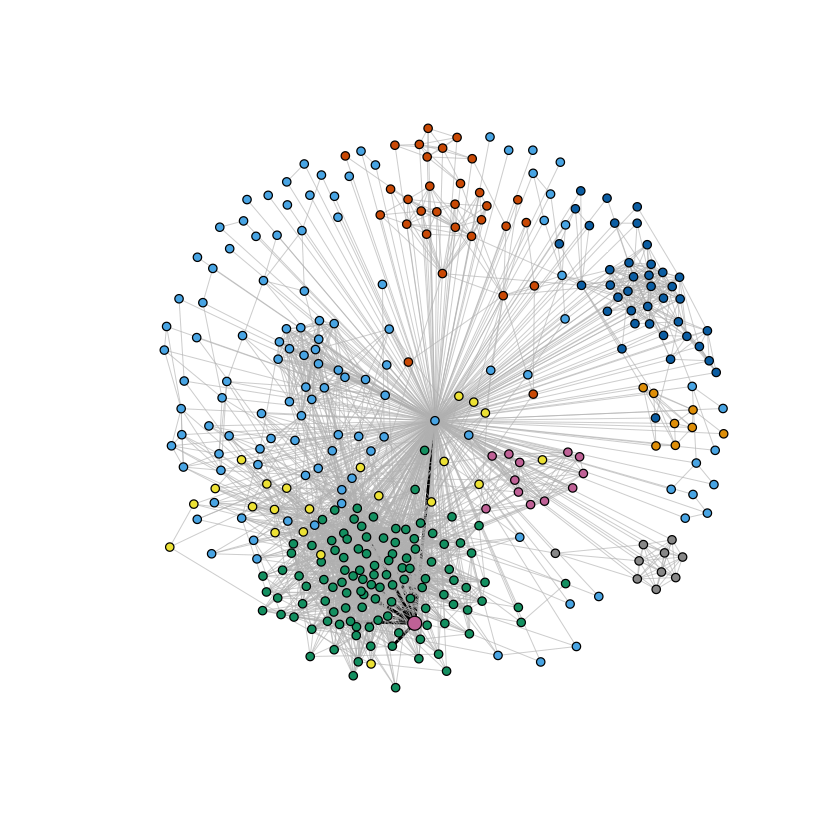
\includegraphics{Figures/1_3_4_1.png}}
\caption{The community structure of No. 1}
\label{1_3_4_1}
\end{minipage}
\begin{minipage}[t]{0.48\textwidth}
\centering
\scalebox{1}{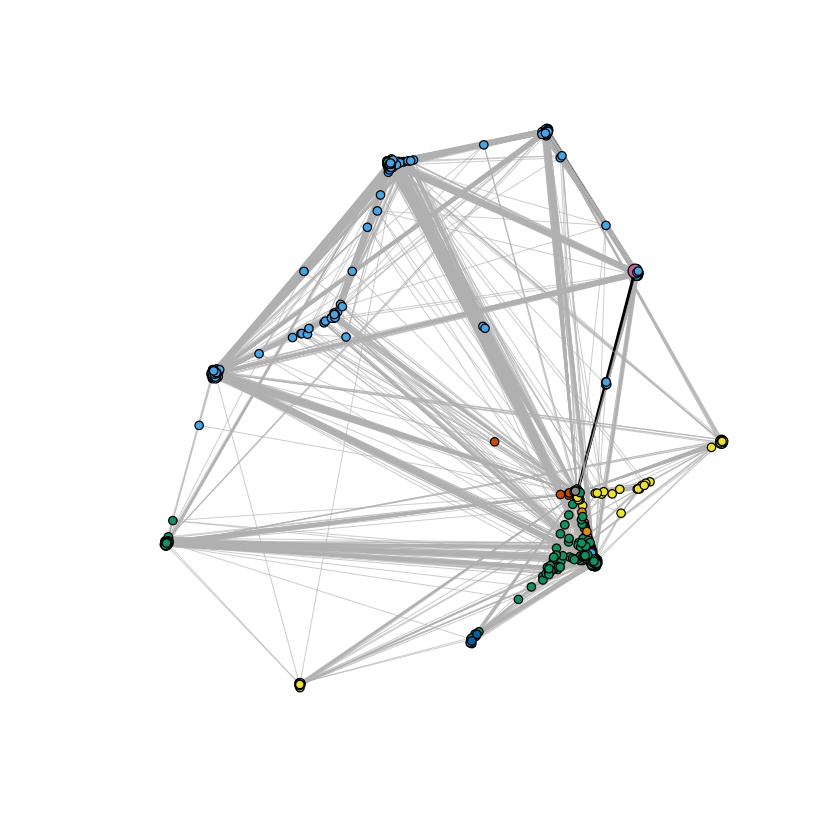
\includegraphics{Figures/1_3_4_2.png}}
\caption{TThe community structure of No. 108}
\label{1_3_4_2}
\end{minipage}
\end{figure}

\begin{figure}[h]
\centering
\begin{minipage}[t]{0.48\textwidth}
\centering
\scalebox{1}{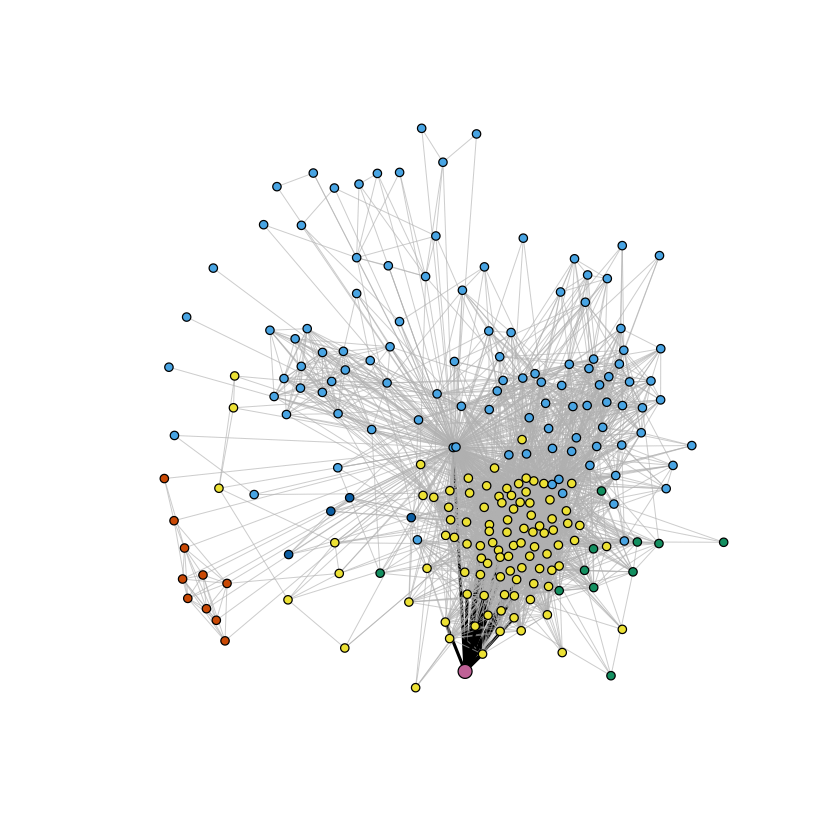
\includegraphics{Figures/1_3_4_3.png}}
\caption{The community structure of No. 349}
\label{1_3_4_3}
\end{minipage}
\begin{minipage}[t]{0.48\textwidth}
\centering
\scalebox{1}{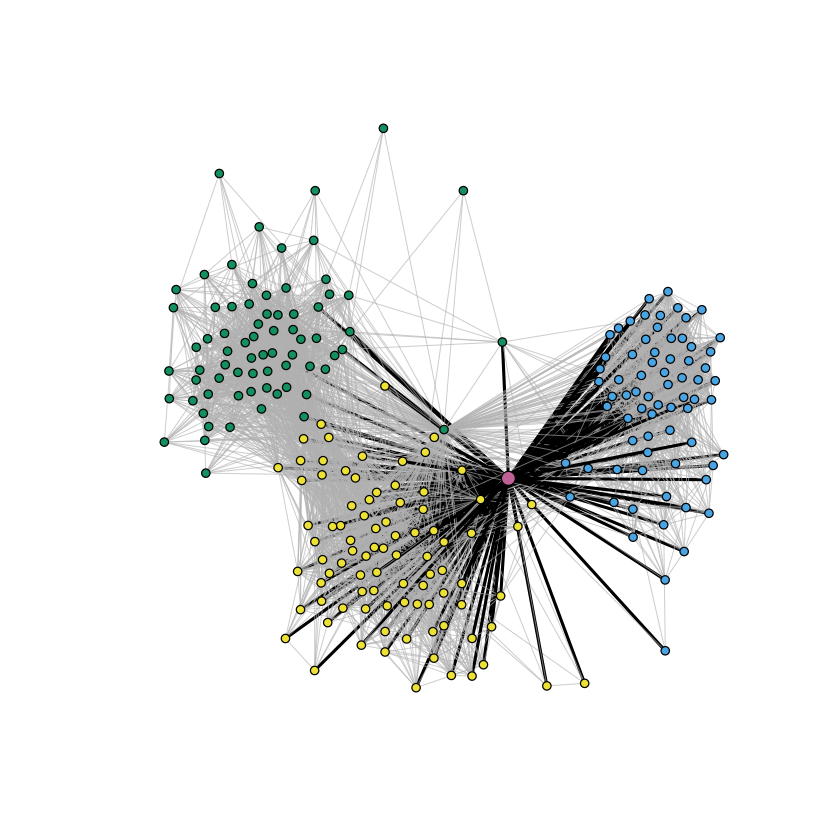
\includegraphics{Figures/1_3_4_4.png}}
\caption{The community structure of No. 484}
\label{1_3_4_4}
\end{minipage}
\end{figure}
\begin{figure}[h]
\centering
\scalebox{0.5}{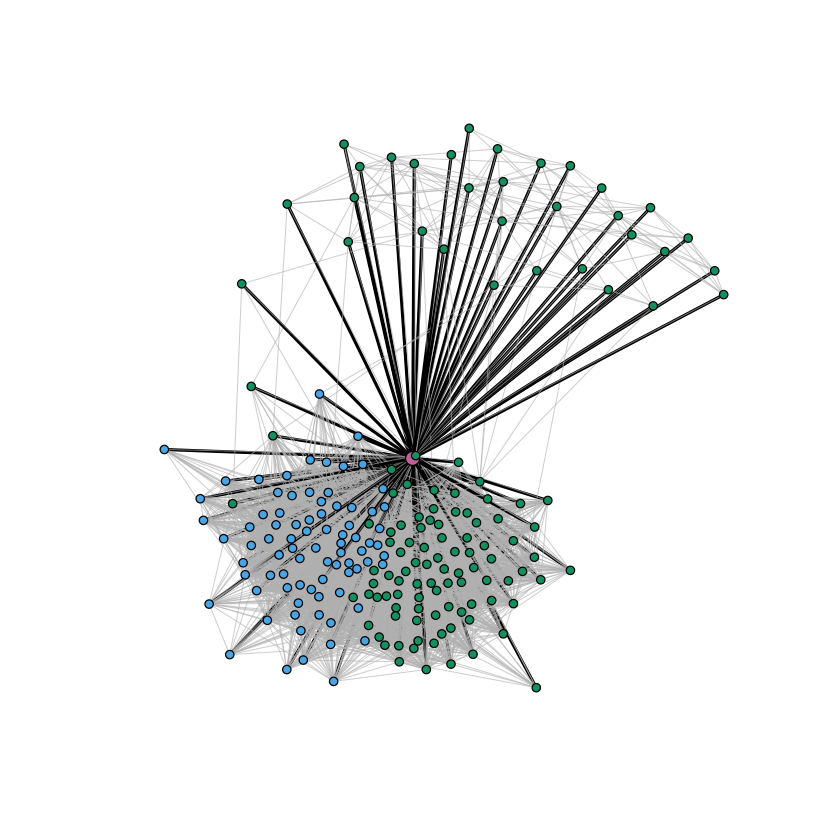
\includegraphics{Figures/1_3_4_5.png}}
\caption{The community structure of No. 1087}
\label{1_3_4_5}
\end{figure}

Similarly, this time we highlight the node with maximum embeddedness and the node with maximum ratio of dispersion to embeddedness. 

For code code 1’s personalized network, the community structure is shown in Fig \ref{1_3_4_6}.
For code code 108’s personalized network, the community structure is shown in Fig \ref{1_3_4_7}.
For code code 349’s personalized network, the community structure is shown in Fig \ref{1_3_4_8}.
For code code 484’s personalized network, the community structure is shown in Fig \ref{1_3_4_9}.
For code code 1087’s personalized network, the community structure is shown in Fig \ref{1_3_4_10}.

\begin{figure}[h]
\centering
\begin{minipage}[t]{0.48\textwidth}
\centering
\scalebox{1}{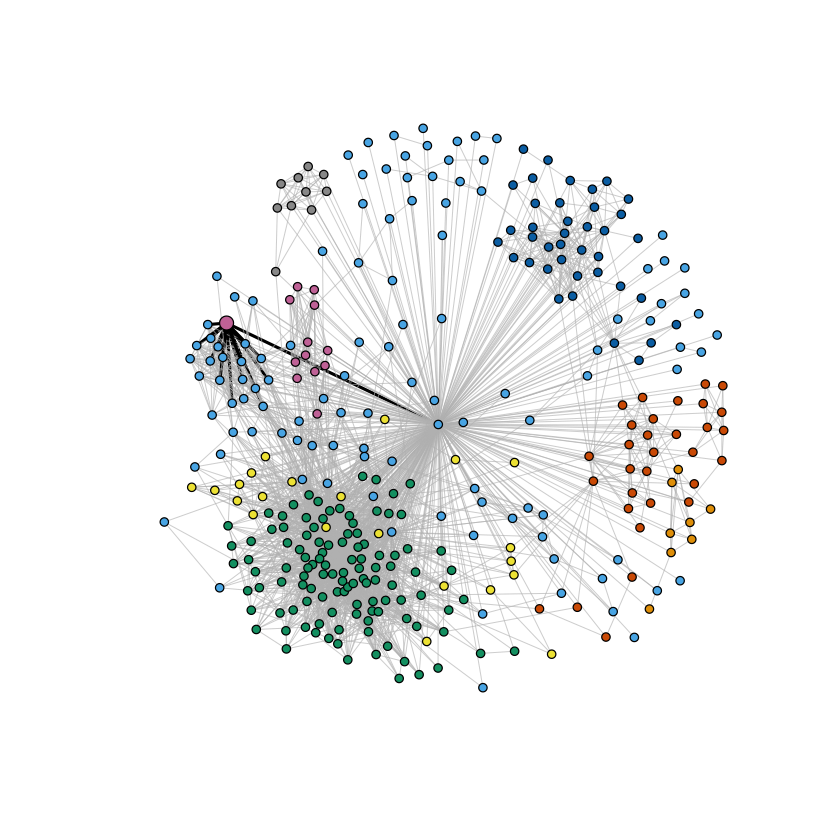
\includegraphics{Figures/1_3_4_6.png}}
\caption{The community structure of No. 1}
\label{1_3_4_6}
\end{minipage}
\begin{minipage}[t]{0.48\textwidth}
\centering
\scalebox{1}{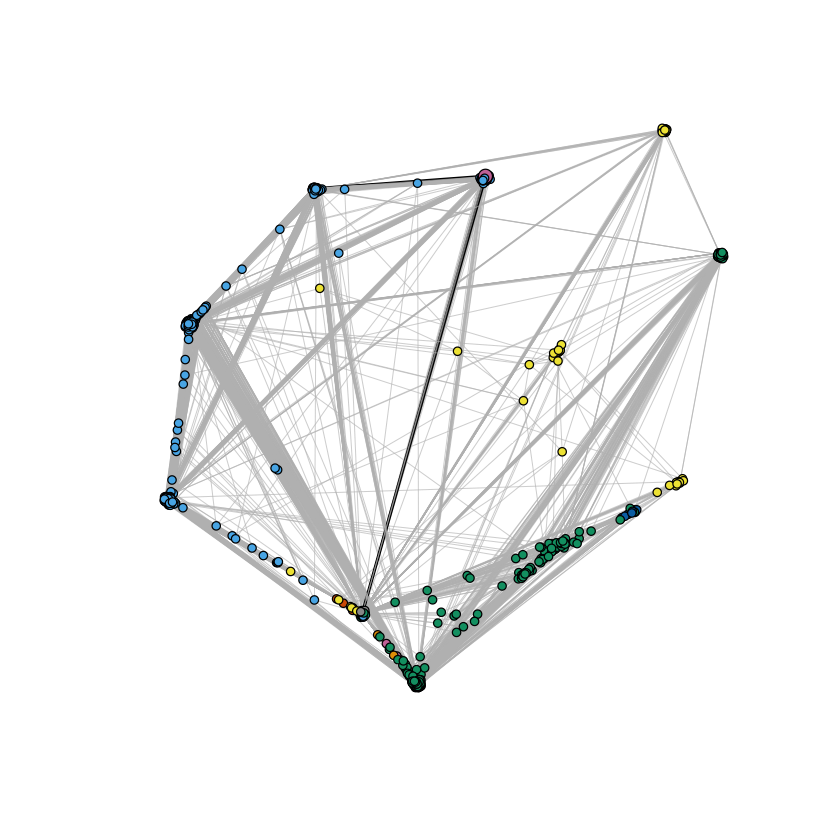
\includegraphics{Figures/1_3_4_7.png}}
\caption{TThe community structure of No. 108}
\label{1_3_4_7}
\end{minipage}
\end{figure}

\begin{figure}[h]
\centering
\begin{minipage}[t]{0.48\textwidth}
\centering
\scalebox{1}{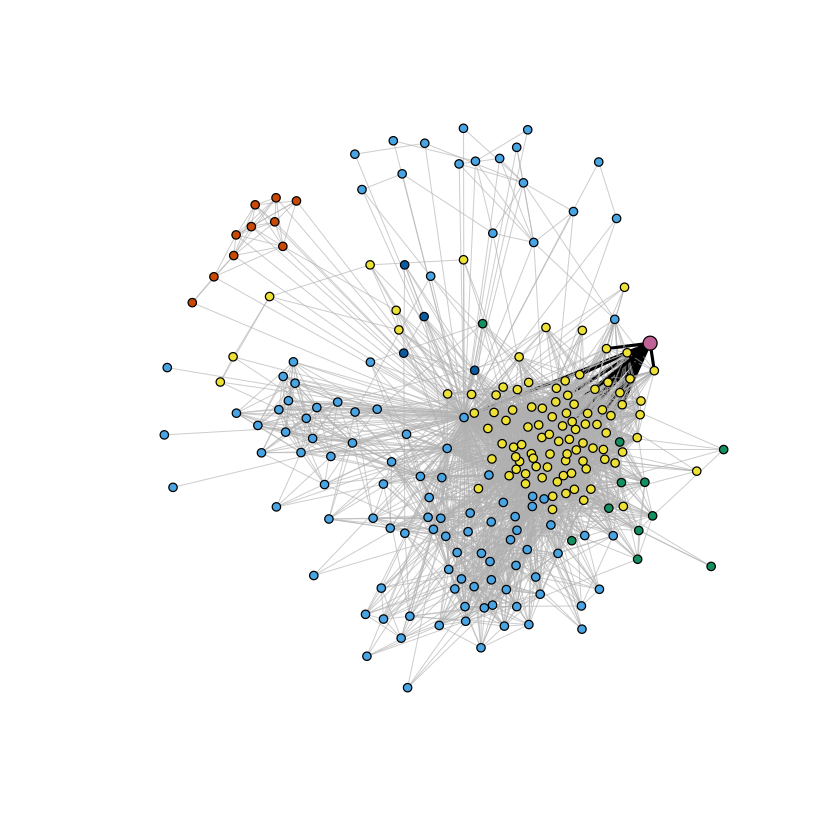
\includegraphics{Figures/1_3_4_8.png}}
\caption{The community structure of No. 349}
\label{1_3_4_8}
\end{minipage}
\begin{minipage}[t]{0.48\textwidth}
\centering
\scalebox{1}{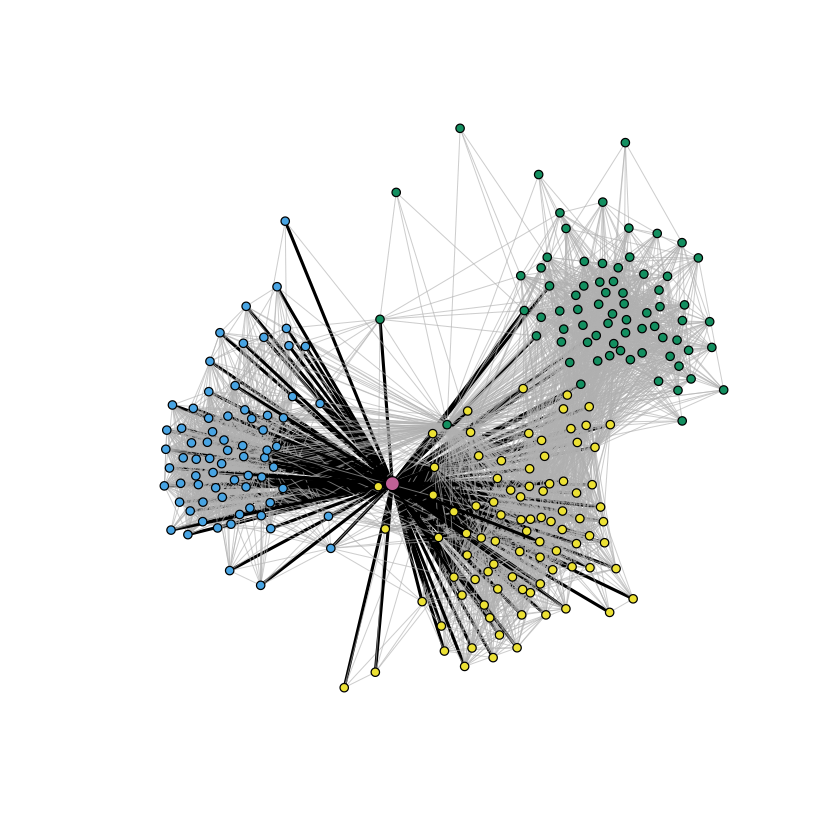
\includegraphics{Figures/1_3_4_9.png}}
\caption{The community structure of No. 484}
\label{1_3_4_9}
\end{minipage}
\end{figure}
\begin{figure}[h]
\centering
\scalebox{0.5}{\includegraphics{Figures/1_3_4_10.png}}
\caption{The community structure of No. 1087}
\label{1_3_4_10}
\end{figure}



\subsection{Friend recommendation in personalized networks}

\subsubsection{Neighborhood based measure}


\subsubsection{Friend recommendation using neighborhood based measures}

\subsubsection{Creating the list of users}

\subsubsection{Average accuracy of friend recommendation algorithm}





\section{Google+ Network}

\subsection{Community structure of personal networks}




\end{document}







